Chương này trình bày quá trình phân tích và thiết kế kiến trúc hệ thống GraphRAG phục vụ việc khai thác tri thức trong lĩnh vực nghệ thuật Chèo. Trên cơ sở các nền tảng lý thuyết đã trình bày ở Chương 2, chương này tập trung mô tả cách thức xây dựng Knowledge Graph và tích hợp nó với mô hình ngôn ngữ lớn nhằm xây dựng một hệ thống hỏi đáp có khả năng khai thác tri thức có cấu trúc và hỗ trợ suy luận đa bước. Nội dung chương 3 bao gồm mô tả kiến trúc tổng thể của hệ thống và phân tích các thành phần chính như tầng tri thức (Knowledge Layer), phân hệ truy xuất đồ thị (G-Retrieval) và phân hệ tạo sinh (G-Generation), qua đó làm rõ cấu trúc và cơ chế vận hành của hệ thống GraphRAG được đề xuất.
\section{Tổng quan kiến trúc hệ thống}
\subsection{Yêu cầu thiết kế hệ thống}
Hệ thống GraphRAG trong nghiên cứu này được thiết kế dựa trên một tập hợp các yêu cầu nhằm đảm bảo khả năng khai thác tri thức hiệu quả trong miền nghệ thuật Chèo. Các yêu cầu này được phân thành hai nhóm chính, bao gồm \textit{yêu cầu chức năng} và \textit{yêu cầu phi chức năng}. Nhóm yêu cầu chức năng tập trung vào việc nâng cao chất lượng truy xuất và suy luận tri thức, trong khi nhóm yêu cầu phi chức năng hướng đến việc đảm bảo tính linh hoạt, ổn định và khả năng mở rộng của hệ thống.

Về mặt chức năng, hệ thống GraphRAG cần đảm bảo ba yêu cầu cốt lõi bao gồm: (i) \textit{độ chính xác tri thức}, (ii) \textit{khả năng suy luận đa bước} và (iii) \textit{khả năng khai thác cấu trúc quan hệ trong Knowledge Graph}. Để đảm bảo độ chính xác tri thức, hệ thống được thiết kế theo hướng kết hợp giữa truy xuất có cấu trúc từ Knowledge Graph và cơ chế xây dựng ngữ cảnh đầu vào có kiểm soát cho mô hình ngôn ngữ. Cụ thể, các thực thể và quan hệ được lựa chọn dựa trên truy vấn và ràng buộc ngữ nghĩa trong đồ thị, thay vì phụ thuộc hoàn toàn vào độ tương đồng ngữ nghĩa như trong các phương pháp truy xuất văn bản truyền thống, qua đó giảm thiểu hiện tượng nhiễu và sai lệch thông tin. Tiếp theo, nhằm đáp ứng yêu cầu suy luận đa bước, hệ thống triển khai cơ chế duyệt đồ thị theo nhiều bước kết hợp với các luật suy luận ở mức ứng dụng, cho phép mở rộng truy vấn ban đầu thành chuỗi các truy vấn con và thu thập tri thức từ nhiều thực thể trung gian. Cách tiếp cận này giúp mô hình không chỉ truy xuất thông tin trực tiếp mà còn có khả năng tổng hợp và liên kết tri thức phân tán. Cuối cùng, để khai thác hiệu quả cấu trúc quan hệ, tri thức được biểu diễn dưới dạng đồ thị và hệ thống áp dụng các chiến lược truy xuất dựa trên cạnh (edge-based retrieval), từ đó cho phép phát hiện và tận dụng các mối liên kết ngữ nghĩa phức tạp mà các phương pháp dựa trên văn bản thuần túy khó có thể khai thác.

Về mặt phi chức năng, hệ thống cần đảm bảo ba yêu cầu bao gồm: (i) tính độc lập với mô hình ngôn ngữ lớn, (ii) hiệu năng và độ ổn định trong truy xuất – suy luận, và (iii) khả năng mở rộng – tái sử dụng. Trước hết, nhằm đảm bảo tính độc lập và giảm sự phụ thuộc vào các nhà cung cấp LLMs, hệ thống được thiết kế theo hướng LLM-agnostic, trong đó mô hình ngôn ngữ chỉ đóng vai trò sinh ngôn ngữ dựa trên ngữ cảnh đã được truy xuất và cấu trúc hóa, không tham gia vào quá trình lưu trữ hay học tri thức miền. Một lớp trung gian chịu trách nhiệm điều phối prompt và chuẩn hóa đầu vào – đầu ra được sử dụng để đảm bảo khả năng thay thế mô hình mà không ảnh hưởng đến logic hệ thống. Bên cạnh đó, do đặc thù của GraphRAG liên quan đến các truy vấn đa bước trên đồ thị, hệ thống cần đảm bảo hiệu năng và độ ổn định trong quá trình truy xuất và suy luận, bao gồm việc tối ưu hóa quá trình duyệt đồ thị, kiểm soát độ trễ và giới hạn kích thước ngữ cảnh đưa vào mô hình nhằm duy trì khả năng phản hồi trong thời gian thực. Cuối cùng, để hỗ trợ khả năng mở rộng và tái sử dụng, hệ thống được xây dựng theo kiến trúc phân tầng, tách biệt giữa tầng dữ liệu (Knowledge Graph), tầng xử lý GraphRAG, và tầng mô hình ngôn ngữ, cho phép tích hợp thêm nguồn tri thức mới, mở rộng ontology hoặc cải tiến chiến lược truy xuất mà không làm ảnh hưởng đến các thành phần hiện có.

\subsection{Kiến trúc phân tầng của hệ thống}
Hệ thống GraphRAG được thiết kế theo kiến trúc phân tầng (layered architecture) (Hình \ref{fig:4-layer}) nhằm tách biệt các chức năng chính của hệ thống và đảm bảo khả năng mở rộng cũng như bảo trì trong quá trình phát triển. Trong mô hình này, hệ thống được chia thành bốn tầng chính gồm: (i) tầng giao diện người dùng (User Interface Layer), (ii) tầng xử lý GraphRAG (GraphRAG Processing Layer), (iii) tầng tri thức (Knowledge Layer) và (iv) tầng mô hình ngôn ngữ (LLM Layer). Việc phân tách này giúp kiểm soát rõ ràng vai trò của từng thành phần trong quá trình tiếp nhận truy vấn, truy xuất tri thức và tạo sinh câu trả lời.

\textbf{Tầng giao diện người dùng} đóng vai trò là cầu nối tương tác giữa người dùng và hệ thống. Tầng này chịu trách nhiệm tiếp nhận truy vấn từ người dùng, hiển thị kết quả trả lời và cung cấp môi trường trực quan để quan sát kết quả suy luận của hệ thống. Tầng giao diện có nhiệm vụ đảm bảo khả năng sử dụng của hệ thống, hỗ trợ người dùng khai thác tri thức về nghệ thuật Chèo thông qua giao diện trực quan và các truy vấn ngôn ngữ tự nhiên.

\textbf{Tầng xử lý GraphRAG} đóng vai trò trung tâm của hệ thống GraphRAG, chịu trách nhiệm tổ chức và điều khiển toàn bộ luồng xử lý truy vấn. Khi nhận được câu hỏi từ người dùng, tầng này thực hiện các bước phân tích truy vấn, gọi các mô-đun truy xuất tri thức từ Knowledge Graph, thực hiện các bước chuyển đổi định dạng dữ liệu và cuối cùng gửi ngữ cảnh đã được xử lý đến LLMs. Tầng xử lý GraphRAG đóng vai trò kết nối giữa tầng tri thức và tầng mô hình ngôn ngữ, góp phần đảm bảo các thành phần khác của hệ thống hoạt động một cách phối hợp và thống nhất.

\textbf{Tầng tri thức} là nơi lưu trữ và quản lý toàn bộ tri thức của hệ thống dưới dạng Knowledge Graph. Trong hệ thống được đề xuất, tri thức về nghệ thuật Chèo được tổ chức thành các thực thể và quan hệ trong đồ thị, cho phép biểu diễn các mối liên hệ phức tạp giữa vở diễn, nhân vật, vai diễn và các yếu tố nghệ thuật khác. Ngoài chức năng lưu trữ dữ liệu, tầng này còn bao gồm các cơ chế đánh chỉ mục và suy luận nhằm hỗ trợ quá trình truy xuất tri thức. Nhờ cấu trúc đồ thị, hệ thống có thể mở rộng ngữ cảnh thông qua quan hệ giữa thực thể và hỗ trợ các truy vấn yêu cầu suy luận đa bước.

\textbf{Tầng mô hình ngôn ngữ} cung cấp năng lực xử lý ngôn ngữ cho hệ thống thông qua API của nhà cung cấp mô hình AI. Trong hệ thống GraphRAG được đề xuất, LLMs không chỉ được sử dụng trong giai đoạn sinh câu trả lời mà còn hỗ trợ một số bước xử lý truy vấn trong tầng xử lý GraphRAG. LLMs được sử dụng để phân tích câu hỏi của người dùng, trích xuất các thực thể và thông tin cần thiết, điền chúng vào các mẫu truy vấn đã được định nghĩa trước nhằm thực hiện truy vấn trên Knowledge Graph. Sau khi truy xuất thu được ngữ cảnh phù hợp từ đồ thị tri thức, LLMs tiếp tục được sử dụng để tổng hợp và sinh câu trả lời dưới dạng ngôn ngữ tự nhiên dựa trên ngữ cảnh đã được cung cấp.

Trong kiến trúc hệ thống, hai tầng đóng vai trò cốt lõi là tầng tri thức và tầng xử lý GraphRAG. Tầng tri thức chịu trách nhiệm lưu trữ và tổ chức tri thức miền dưới dạng Knowledge Graph, trong khi tầng xử lý GraphRAG điều phối quá trình truy xuất và xây dựng ngữ cảnh phục vụ mô hình ngôn ngữ. Các tầng còn lại chủ yếu đảm nhận vai trò hỗ trợ, bao gồm giao diện người dùng cho tương tác và tầng mô hình ngôn ngữ được triển khai thông qua các dịch vụ bên ngoài. Do đó, trọng tâm của khóa luận tập trung vào việc phát triển tầng tri thức và các cơ chế xử lý trong tầng GraphRAG, đặc biệt là hai phân hệ G-Retrieval và G-Generation.

\begin{figure}
    \centering
    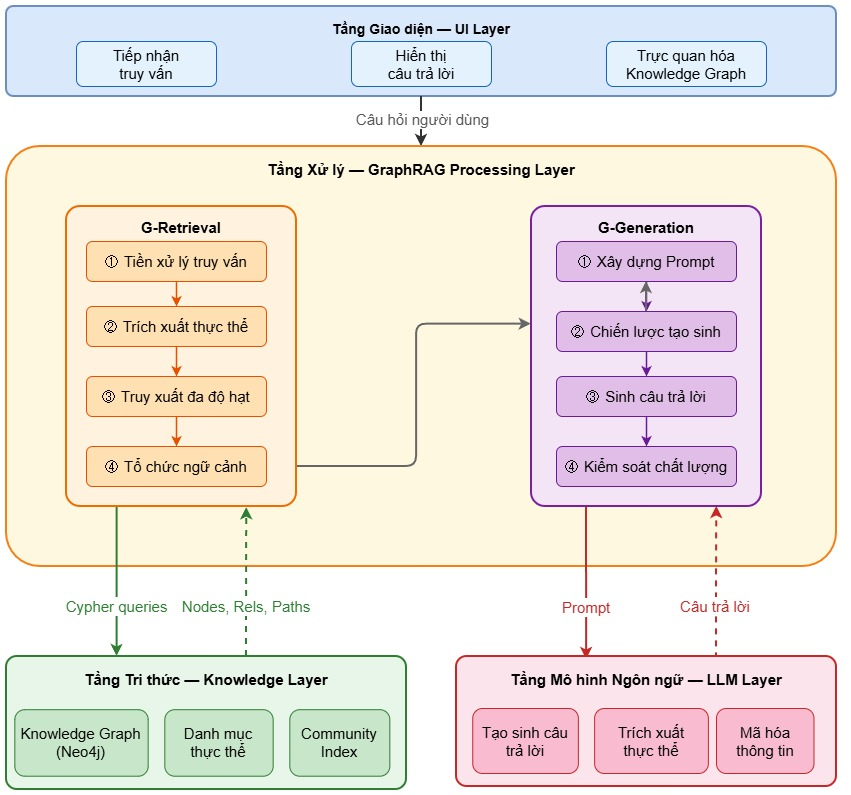
\includegraphics[width=1\linewidth]{figures//c3/4-layer.jpg}
    \caption{Thiết kế 4 tầng của hệ thống GraphRAG}
    \label{fig:4-layer}
\end{figure}

\subsection{Luồng xử lý tổng thể}

Quy trình xử lý của hệ thống (Hình~\ref{fig:overview}) bắt đầu khi người dùng nhập một câu hỏi bằng ngôn ngữ tự nhiên. Câu hỏi được đưa qua phân hệ truy xuất đồ thị (G-Retrieval) để thu thập ngữ cảnh tri thức, sau đó chuyển tới phân hệ tạo sinh (G-Generation) để sinh câu trả lời.

Phân hệ G-Retrieval thực hiện ba bước liên tiếp. Trước tiên, câu hỏi được tiền xử lý thông qua phân tích truy vấn và trích xuất thực thể nhằm xác định các điểm neo trong Knowledge Graph. Tiếp đến, hệ thống thực hiện truy vấn đa mức độ trên đồ thị ở các mức nút (node), bộ ba quan hệ (triplet), đường dẫn quan hệ (path) hoặc đồ thị con (subgraph) tuỳ theo mức độ phức tạp của truy vấn. Cuối cùng, dữ liệu truy xuất được tổ chức thành năm biểu diễn ngữ cảnh phù hợp với mô hình ngôn ngữ: văn bản tự nhiên, bảng kề (adjacency table), cấu trúc JSON (code-like), chuỗi nút (node sequence) và tóm tắt cộng đồng (community summary).

Ngữ cảnh sau khi tổ chức được kết hợp với câu hỏi ban đầu để xây dựng prompt đầu vào cho G-Generation. Phân hệ G-Generation sử dụng mô hình ngôn ngữ lớn để tạo sinh câu trả lời theo ba phương pháp tuỳ cách kiểm soát quá trình sinh: (i) sinh dựa trên ngữ cảnh đã chuẩn bị trước (pre-generation), (ii) sinh có điều hướng trong quá trình suy luận (mid-generation) và (iii) sinh kèm cơ chế kiểm chứng và hiệu chỉnh (post-generation). Ba phương pháp tương ứng với các mức kiểm soát khác nhau, từ xác định ngữ cảnh đầu vào, can thiệp tiến trình suy luận đến đánh giá và điều chỉnh kết quả đầu ra. Toàn bộ quy trình tách biệt giữa truy xuất tri thức và sinh ngôn ngữ: tri thức được xác định và kiểm soát trong G-Retrieval, còn mô hình ngôn ngữ ở G-Generation đóng vai trò tổng hợp lại thông tin và diễn đạt kết quả tới người dùng.

\begin{figure}
    \centering
    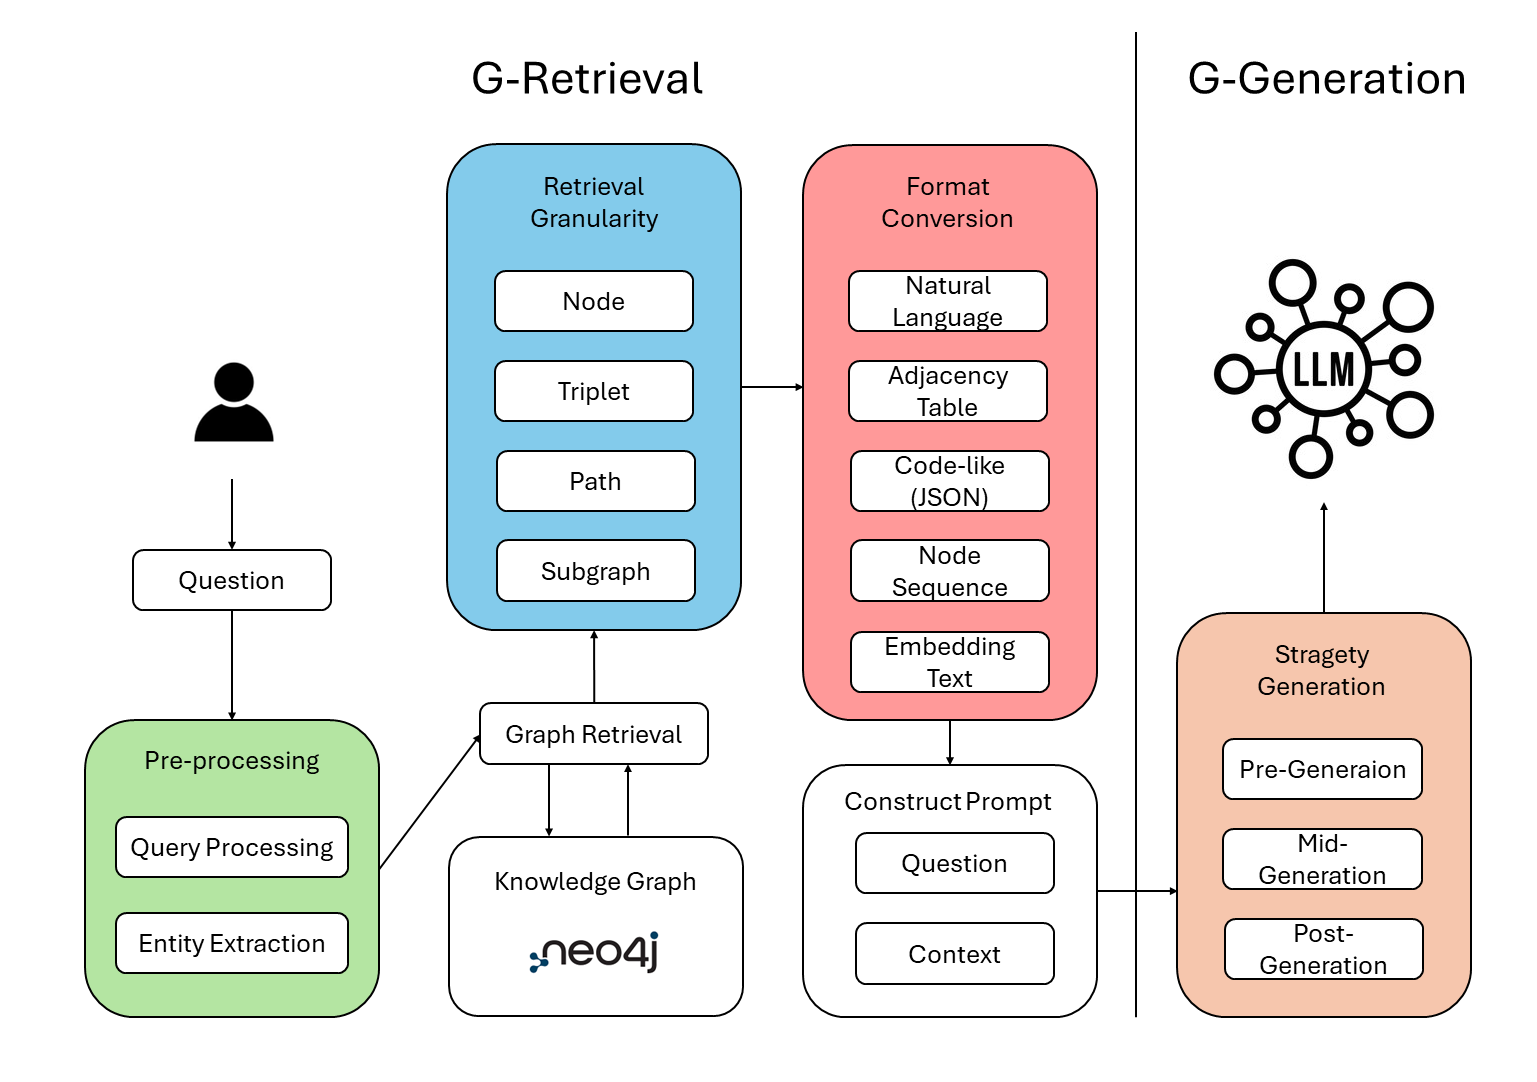
\includegraphics[width=0.9\linewidth]{figures//c3/Slide1.PNG}
    \caption{Tổng quan luồng xử lý GraphRAG}
    \label{fig:overview}
\end{figure}

\section{Thiết kế tầng tri thức}

\subsection{Kế thừa và chuyển đổi Ontology sang Knowledge Graph}

\subsubsection{Ontology Chèo - nền tảng tri thức}

Hệ thống GraphRAG được đề xuất kế thừa ontology về nghệ thuật Chèo xây dựng trong khóa luận tốt nghiệp của chị Trương Quỳnh Giang~\cite{Giang2025}. Ontology được hình thức hóa theo chuẩn OWL, lưu trữ dưới định dạng Turtle (\texttt{.ttl})/OWL (\texttt{.owl}) và phát triển trên nền tảng Protégé, là cơ sở lý thuyết phù hợp để xây dựng nên đồ thị tri thức phục vụ cho hệ thống truy xuất thông tin.

\textbf{Kiến trúc.}
Ontology tổ chức tri thức theo mô hình phân lớp với 7 lớp, 7 thuộc tính quan hệ (object properties) và 17 thuộc tính dữ liệu (data properties). Bảng~\ref{tab:ontology_classes} trình bày từng lớp cùng vai trò ngữ nghĩa và tập thuộc tính dữ liệu tương ứng.

\begin{table}[ht]
  \centering
  \caption{Bảy lớp trong Chèo Ontology và các thuộc tính dữ liệu tương ứng.}
  \label{tab:ontology_classes}
  \renewcommand{\arraystretch}{1.35}
  \small
  \begin{tabular}{p{3.5cm} p{3.3cm} p{7.99cm}}
    \toprule
    \textbf{Lớp} & \textbf{Vai trò} & \textbf{Thuộc tính dữ liệu} \\
    \midrule
    \texttt{Play}
      & Vở chèo
      & \texttt{title}, \texttt{summary}, \texttt{author}, \texttt{sceneNumber} \\[2pt]
    \texttt{Character}
      & Nhân vật trong vở
      & \texttt{charName}, \texttt{description}, \texttt{mainType}, \texttt{subType}, \texttt{charGender} \\[2pt]
    \texttt{Actor}
      & Diễn viên
      & \texttt{actorName}, \texttt{actorGender} \\[2pt]
    \texttt{Scene}
      & Trích đoạn
      & \texttt{sceneName}, \texttt{sceneSummary}, \texttt{versionNumber} \\[2pt]
    \texttt{Version}
      & Phiên bản biểu diễn
      & \texttt{showDate}, \texttt{vidVersion}, \texttt{videoDuration}, \texttt{resolution},
        \texttt{aspectRatio}, \texttt{startTime}, \texttt{endTime}, \texttt{ID} \\[2pt]
    \texttt{RoleAssignment}
      &  Phân công vai diễn
      & --- \\[2pt]
    \texttt{Appearance}
      & Một lần xuất hiện trong video
      & \texttt{start}, \texttt{end}, \texttt{emotion}, \texttt{subtitle}, \texttt{ED} \\
    \bottomrule
  \end{tabular}
\end{table}

Bảy thuộc tính quan hệ tạo thành cấu trúc liên kết giữa các thực thể trong đồ thị: lớp Play kết nối tới Character và Scene qua \texttt{hasCharacter} và \texttt{hasScene}; Scene kết nối tới Version qua \texttt{hasVersion}. Lớp trung gian \texttt{RoleAssignment} kết nối ra ba hướng qua \texttt{performedBy}~(Actor), \texttt{forCharacter}~(Character) và \texttt{inVersion}~(Version), đồng thời nối sang Appearance qua \texttt{hasAppearance}.

\textbf{Độ phủ tri thức.}
Ontology bao quát \textbf{bảy vở chèo} kinh điển trong kho lưu trữ của Trường Đại học Sân khấu – Điện ảnh Hà Nội: Quan Âm Thị Kính, Kim Nham, Trương Viên, Lưu Bình Dương Lễ, Chu Mãi Thần, Từ Thức và Trịnh Nguyên. Tổng cộng \textbf{400 thực thể} (individuals) được định nghĩa tường minh - 7~vở diễn, 38~nhân vật, 41~diễn viên, 15~trích đoạn, 27~phiên bản biểu diễn, 76~phân công vai diễn, cùng tập Appearance ghi nhận thông tin xuất hiện theo khung hình video với độ chi tiết đến từng thời điểm xuất hiện, có gán nhãn cảm xúc và lời thoại. Toàn bộ thực thể được xây dựng từ dữ liệu thực tế của nhà trường, đảm bảo tính xác thực của cơ sở tri thức.

\textbf{Cơ sở kế thừa.}
Với một hệ thống GraphRAG, ontology đáp ứng được ba tiêu chí nền tảng để trở thành nguồn tri thức đáng tin cậy: (i) \textit{chất lượng cơ sở dữ liệu}, (ii) \textit{khả năng mô hình hóa miền thông tin} và (iii) \textit{chiều sâu dữ liệu}. Về chất lượng cơ sở dữ liệu, cấu trúc OWL với ràng buộc domain/range trên từng object property đảm bảo tính nhất quán logic có thể kiểm tra bằng reasoner, loại bỏ các mâu thuẫn ngữ nghĩa ở lớp lưu trữ. Về khả năng mô hình hóa miền, thông qua các lớp \texttt{RoleAssignment} và \texttt{Appearance} biểu diễn được đặc thù của nghệ thuật biểu diễn sống - cùng một trích đoạn có thể được dàn dựng nhiều lần với dàn diễn viên hoàn toàn khác nhau - mà các mô hình quan hệ phẳng không nắm bắt được. Về chiều sâu dữ liệu, thông tin ở mức frame-level trong \texttt{Appearance} tạo nền tảng cho các phân tích vượt ngoài phạm vi truy xuất thực thể đơn thuần, cung cấp được nhiều thông tin hơn về các trích đoạn nhỏ, những nét diễn của từng diễn viên hay đặc điểm của từng nhân vật.

Tuy nhiên, khi đặt trong bối cảnh hệ thống hỏi-đáp thời gian thực, mô hình OWL thuần túy bộc lộ bốn hạn chế kỹ thuật cơ bản, ảnh hưởng trực tiếp đến khả năng đáp ứng về độ trễ và độ chính xác truy xuất:

\begin{enumerate}
\item \textit{Hạn chế trong biểu diễn và tối ưu truy vấn đa bước linh hoạt.}
Mặc dù SPARQL hỗ trợ property path, việc biểu diễn các truy vấn đa bước với độ sâu biến đổi trong thực tế vẫn gặp khó khăn, đặc biệt khi cần kiểm soát và tối ưu hóa hiệu năng. Các truy vấn dạng chuỗi quan hệ dài thường dẫn đến cấu trúc truy vấn phức tạp và khó mở rộng cho các độ sâu khác nhau.

\item \textit{Chi phí suy luận ngữ nghĩa cao, không phù hợp cho thời gian thực.}
Việc khai thác các quan hệ gián tiếp thông qua OWL reasoner có chi phí tính toán lớn, đặc biệt khi áp dụng trên đồ thị có kích thước lớn. Trong các hệ thống yêu cầu phản hồi nhanh, việc thực hiện suy luận tại thời điểm truy vấn là không khả thi, đòi hỏi phải chuyển sang các cơ chế tiền xử lý hoặc lưu trữ suy luận.

\item \textit{Khả năng tối ưu truy vấn theo thuộc tính văn bản còn hạn chế.}
Các truy vấn tìm kiếm theo tên trong SPARQL, thường được thực hiện thông qua \texttt{FILTER} kết hợp với \texttt{REGEX}, không được tối ưu hóa ở mức lưu trữ, dẫn đến chi phí quét toàn bộ dữ liệu trong nhiều trường hợp, đặc biệt với các thuộc tính thường xuyên xuất hiện trong truy vấn người dùng.

\item \textit{Thiếu cơ chế tìm kiếm toàn văn tích hợp ở mức chuẩn.}
OWL/SPARQL không cung cấp sẵn các cơ chế tìm kiếm toàn văn như so khớp không phân biệt hoa–thường hay fuzzy matching, trong khi đây là yêu cầu phổ biến trong các hệ thống hỏi–đáp dựa trên ngôn ngữ tự nhiên, đặc biệt với dữ liệu tên riêng có nhiều biến thể biểu diễn.
\end{enumerate}

Các hạn chế (1) và (2) ảnh hưởng trực tiếp đến khả năng truy xuất và suy luận đa bước trong thời gian thực, trong khi (3) và (4) tác động đến độ chính xác và hiệu năng của các truy vấn dựa trên thuộc tính văn bản. Những phân tích này là cơ sở kỹ thuật quan trọng dẫn đến quyết định chuyển đổi sang mô hình property graph trên Neo4j, nhằm đảm bảo hiệu năng truy xuất mà vẫn duy trì được cấu trúc ngữ nghĩa của ontology ban đầu.

\subsubsection{Chuyển đổi sang Knowledge Graph trên Neo4j}

Quyết định chuyển đổi sang mô hình property graph trên Neo4j nhằm khắc phục các hạn chế về hiệu năng và truy xuất đa bước của SPARQL trong bối cảnh thời gian thực. Cụ thể, Cypher hỗ trợ truy vấn đường đi với độ sâu linh hoạt, trong khi cơ chế indexing ở mức cơ sở dữ liệu giúp giảm phụ thuộc vào suy luận OWL tốn kém và tối ưu hóa các truy vấn theo thuộc tính văn bản, bao gồm cả tìm kiếm không phân biệt hoa–thường. Mặc dù thay đổi mô hình lưu trữ, cấu trúc ngữ nghĩa của ontology vẫn được bảo toàn thông qua việc ánh xạ mỗi OWL class thành node label và mỗi object property thành relationship type; quy trình chuyển đổi từ tệp Turtle sang Chèo Knowledge Graph trên Neo4j được minh họa trong Hình~\ref{fig:ontology_conversion}.

\begin{figure}[ht]
  \centering
  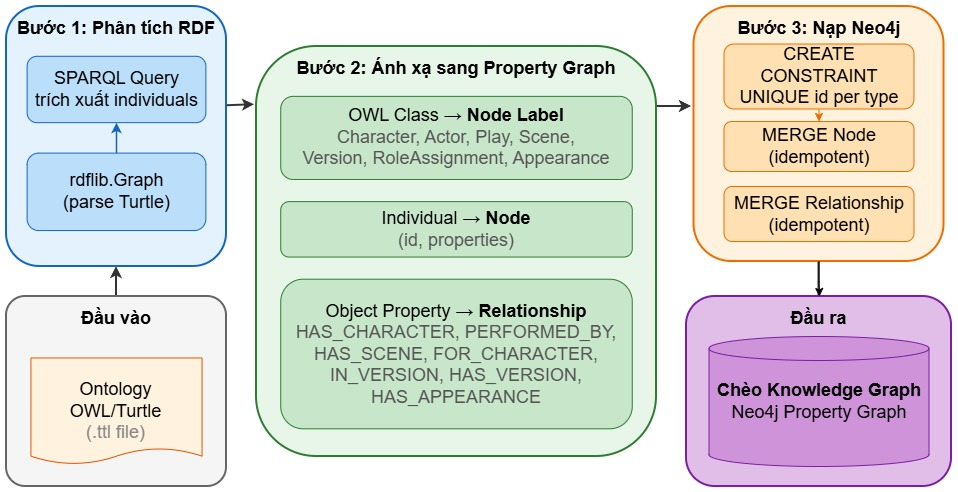
\includegraphics[width=\textwidth]{figures/c3/ontology_conversion.jpg}
  \caption{Quy trình chuyển đổi Ontology OWL~2 sang Knowledge Graph.}
  \label{fig:ontology_conversion}
\end{figure}

\textbf{Bước 1 - Phân tích RDF.}
Hệ thống sử dụng thư viện \texttt{rdflib} để phân tích tệp Turtle thành đồ thị RDF,
sau đó thực hiện truy vấn SPARQL để trích xuất toàn bộ individuals cùng kiểu lớp và
giá trị thuộc tính.

\textbf{Bước 2 - Ánh xạ sang Property Graph.}
Quy tắc ánh xạ được xác định như sau:
\begin{itemize}
  \item Mỗi OWL class $\rightarrow$ một nhãn nút (node label) trong Neo4j.
  \item Mỗi individual $\rightarrow$ một nút với các data properties ánh xạ thành node properties.
  \item Bảy object property $\rightarrow$ bảy loại cạnh quan hệ có hướng.
\end{itemize}

\textbf{Bước 3 - Nạp vào Neo4j.}
Dữ liệu được nạp sử dụng phép \texttt{MERGE} (thay vì \texttt{CREATE}) nhằm đảm bảo
tính idempotent - quá trình nạp có thể chạy lại nhiều lần mà không tạo dữ liệu trùng lặp.
Trước khi nạp, hệ thống thiết lập \texttt{UNIQUE} constraints cho thuộc tính \texttt{id}
của từng loại nút.

Kết quả là một Chèo Knowledge Graph giữ nguyên toàn bộ độ phủ và tính chính xác ngữ nghĩa
của ontology gốc, đồng thời khắc phục các nhược điểm về truy vấn nhờ cơ chế Cypher path
traversal, native indexing và full-text search của Neo4j.

\subsection{Mở rộng và chuẩn hóa lược đồ tri thức}

Knowledge Graph được tạo ra từ Ontology gốc đã bao phủ được khái quát các tri thức của nghệ thuật Chèo, nhưng chưa đáp ứng đầy đủ yêu cầu của hai lớp truy vấn đặc thù trong kiến trúc GraphRAG: (i) truy vấn phân loại thực thể theo loại vai diễn và (ii) truy vấn phân tích yếu tố biểu diễn. Mục này trình bày quá trình mở rộng các phân lớp con từ các phân lớp cha (Bảng \ref{tab:schema_extension}) để xây dựng nên một Knowledge Graph mới, phục vụ khả năng truy vấn và tìm kiếm thông tin linh hoạt và nhanh chóng (Hình \ref{fig:kg_schema})

\textbf{Mở rộng phân lớp nhân vật.}
Trong ontology gốc, loại vai diễn được biểu diễn qua hai thuộc tính dữ liệu
\texttt{mainType} và \texttt{subType} với các giá trị chuỗi (Đào, Kép, Hề, Lão, Mụ). Cách biểu diễn thuộc tính phẳng này buộc tầng truy xuất phải thực hiện lọc tại thời điểm truy vấn (\texttt{WHERE n.mainType = `Đào'}) thay vì nhận dạng trực tiếp qua nhãn nút (\texttt{MATCH (n:Main\_Character)}). Trong pipeline GraphRAG, các truy vấn Cypher được sinh tự động từ ngôn ngữ tự nhiên dựa tên các nhãn nút; việc phân loại thuộc tính làm suy yếu khả năng ánh xạ chính xác từ câu hỏi người dùng sang đồ thị. Lớp \texttt{Character} do đó được mở rộng thành ba lớp con:

\begin{itemize}
  \item \texttt{Main\_Character} - nhân vật chính diện giữ vai trò trung tâm trong
    cốt truyện, tương ứng với loại Đào (nữ chính) và Kép (nam chính) trong hệ thống
    phân loại nhân vật Chèo truyền thống.
  \item \texttt{Supporting\_Character} - nhân vật phụ trong các cảnh hỗ trợ hoặc
    hài, bao gồm các loại Hề, Lão và Mụ.
  \item \texttt{Antagonist} - nhân vật đối lập tạo xung đột kịch tính, có chức
    năng phản diện rõ ràng trong tuyến truyện (Sùng Bà, Trần Phương, Đào Huế...).
\end{itemize}

\textbf{Mở rộng phân loại biểu diễn.}
Lớp \texttt{Appearance} trong ontology gốc lưu trữ toàn bộ thông tin xuất hiện của
nhân vật theo khung hình dưới dạng thực thể duy nhất mà không phân biệt thể loại biểu
đạt. Với hệ thống hỏi-đáp có thể nhận câu hỏi về từng loại yếu tố biểu diễn, lớp
\texttt{Appearance} được phân thành ba nhóm con độc lập về ngữ nghĩa:

\begin{itemize}
  \item \texttt{Physical\_Gesture} - chuyển động thân thể trong diễn xuất; được
    phân chi tiết thành \texttt{Hand\_Gesture} (cử chỉ tay) và
    \texttt{Leg\_Movement} (bộ chân).
  \item \texttt{Costume\_Artifact} - yếu tố trang phục và đạo cụ sân khấu gắn
    với từng lần xuất hiện của nhân vật.
  \item \texttt{Vocal\_Expression} - biểu đạt thanh nhạc và lời hát; hỗ trợ
    phân tích phong cách diễn xướng theo từng loại vai.
\end{itemize}

\begin{table}[ht]
  \centering
  \caption{Tám lớp con bổ sung trong Chèo Knowledge Graph}
  \label{tab:schema_extension}
  \renewcommand{\arraystretch}{1.3}
  \footnotesize
  \begin{tabular}{p{4.0cm} p{3.2cm} p{7.59cm}}
    \toprule
    \textbf{Lớp con} & \textbf{Lớp cha} & \textbf{Ngữ nghĩa và vai trò thiết kế} \\
    \midrule
    \texttt{Main\_Character}
      & \texttt{Character}
      & Nhân vật Đào/Kép; truy vấn phân loại vai chính qua nhãn nút. \\[2pt]
    \texttt{Supporting\_Character}
      & \texttt{Character}
      & Nhân vật Hề/Lão/Mụ; phân biệt ngữ nghĩa với nhân vật chính ở lớp
        nhãn đồ thị. \\[2pt]
    \texttt{Antagonist}
      & \texttt{Character}
      & Nhân vật phản diện; hỗ trợ truy vấn phân tích tuyến xung đột
        kịch tính. \\[4pt]
    \texttt{Physical\_Gesture}
      & \texttt{Appearance}
      & Lớp cha trung gian cho chuyển động thân thể; nhóm \texttt{Hand\_Gesture}
        và \texttt{Leg\_Movement}. \\[2pt]
    \texttt{Hand\_Gesture}
      & \texttt{Physical\_Gesture}
      & Cử chỉ tay --- yếu tố múa đặc trưng theo từng loại vai Chèo. \\[2pt]
    \texttt{Leg\_Movement}
      & \texttt{Physical\_Gesture}
      & Bộ chân --- kỹ thuật di chuyển sân khấu theo phong cách từng nhân vật. \\[2pt]
    \texttt{Costume\_Artifact}
      & \texttt{Appearance}
      & Trang phục và đạo cụ sân khấu; phân biệt với biểu đạt thân thể và
        thanh nhạc. \\[2pt]
    \texttt{Vocal\_Expression}
      & \texttt{Appearance}
      & Biểu đạt thanh nhạc; hỗ trợ phân tích phong cách diễn xướng theo
        loại vai. \\
    \bottomrule
  \end{tabular}
\end{table}

\begin{figure}[!ht]
  \centering
  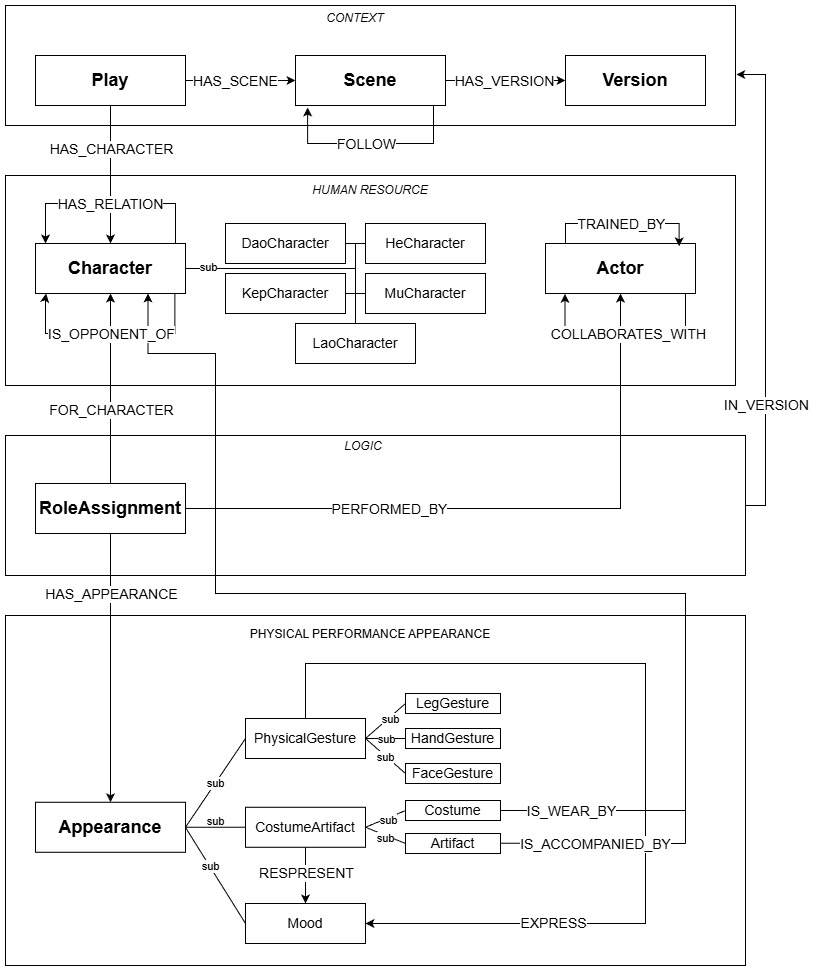
\includegraphics[width=\textwidth]{figures/c3/Ontology2.jpg}
  \caption{Lược đồ Chèo Knowledge Graph sau mở rộng}
  \label{fig:kg_schema}
\end{figure}

% ============================================================

\subsection{Suy luận quan hệ gián tiếp}

Đồ thị sau mở rộng lược đồ chứa toàn bộ tri thức tường minh của miền, nhưng nhiều
câu hỏi thực tế đòi hỏi khai thác \textit{tri thức ngầm} --- các quan hệ không tồn
tại dưới dạng cạnh trực tiếp mà phải suy ra qua chuỗi liên kết nhiều bước. Tùy theo
tần suất và chi phí, hai chiến lược được áp dụng: (i) \textit{mô hình hóa} trước các
quan hệ tần suất cao vào đồ thị như cạnh tường minh, và (ii) \textit{suy luận động} tại
runtime qua biểu thức path Cypher \texttt{*1..\textit{n}~hops} cho các quan hệ còn lại.

\textbf{Mô hình hóa quan hệ.}
Phân tích tập câu hỏi thường gặp cho thấy mẫu ``diễn viên~$x$ tham gia vở nào?''
có tần suất cao nhất. Trong đồ thị gốc, không tồn tại cạnh trực tiếp Actor--Play;
mỗi truy vấn phải duyệt chuỗi bốn bước:

\begin{multline}
  \texttt{Actor} \xrightarrow{\texttt{performedBy}^{-1}}
  \texttt{RoleAssignment} \xrightarrow{\texttt{inVersion}}
  \texttt{Version} \\
  \xrightarrow{\texttt{hasVersion}^{-1}}
  \texttt{Scene} \xrightarrow{\texttt{hasScene}^{-1}}
  \texttt{Play}
  \label{eq:chain_actor_play}
\end{multline}

Quan hệ \texttt{isPerformedIn}~(Actor\,$\to$\,Play) được vật chất hóa bằng cách
thực thi chuỗi~\eqref{eq:chain_actor_play} một lần tại thời điểm xây dựng đồ thị
và lưu kết quả như cạnh tường minh. Chi phí lưu trữ tuyến tính $O(|A||P|)$ - được tính bằng tích số lượng diễn viên và số lượng vở chèo--- được tối ưu chỉ còn là chi phí truy vấn hằng số $O(1)$ cho mẫu tần suất cao này.

Ba chuỗi suy luận động được xác định cho các truy vấn không thể mô hình hóa trước do phụ thuộc vào tham số đầu vào hoặc yêu cầu kèm thông tin trung gian:

\textbf{Chuỗi~1 --- Nhân vật tới diễn viên đảm nhận.}
Câu hỏi dạng ``Những diễn viên nào đã từng đóng vai Thị Màu?'' yêu cầu duyệt
ngược qua hai bước : từ \texttt{Character} ngược cạnh \texttt{forCharacter} về \texttt{RoleAssignment}, rồi xuôi theo \texttt{performedBy} tới \texttt{Actor} (Chuỗi ~\eqref{eq:chain_char_actor}):

\begin{equation}
  \texttt{Character} \xleftarrow{\texttt{forCharacter}}
  \texttt{RoleAssignment} \xrightarrow{\texttt{performedBy}}
  \texttt{Actor}
  \label{eq:chain_char_actor}
\end{equation}

\textbf{Chuỗi~2 --- Vở tới tập diễn viên (đường dài).}
Một số câu hỏi tổng hợp yêu cầu liệt kê \textit{tất cả} diễn viên của một vở kèm
thông tin phiên bản hoặc vai cụ thể --- không thể đáp ứng chỉ bằng cạnh
\texttt{isPerformedIn} vốn chỉ lưu quan hệ Actor--Play. Chuỗi đầy đủ bốn bước
từ \texttt{Play} xuống tới từng \texttt{Actor} qua các nút trung gian:

\begin{multline}
  \texttt{Play} \xrightarrow{\texttt{hasScene}}
  \texttt{Scene} \xrightarrow{\texttt{hasVersion}}
  \texttt{Version} \\
  \xleftarrow{\texttt{inVersion}}
  \texttt{RoleAssignment} \xrightarrow{\texttt{performedBy}}
  \texttt{Actor}
  \label{eq:chain_play_actor}
\end{multline}

Đây là chiều đảo ngược của chuỗi~\eqref{eq:chain_actor_play}: khi cần tra cứu
nhanh diễn viên--vở mà không cần chi tiết trung gian, cạnh tắt \texttt{isPerformedIn}
được dùng; khi cần kèm theo nhân vật, phiên bản, hoặc thời điểm biểu diễn, chuỗi
đầy đủ được thực thi.

\textbf{Chuỗi~3 --- Giao tập diễn viên giữa hai vở.}
Câu hỏi dạng ``Những diễn viên nào tham gia đồng thời cả Quan Âm Thị Kính và
Kim Nham?'' yêu cầu thực hiện chuỗi~\eqref{eq:chain_play_actor} độc lập cho
từng vở, rồi lấy giao hai tập \texttt{Actor} trả về. Biểu thức path
\texttt{*1..4} cho phép Neo4j tự tối ưu theo cấu trúc đồ thị thực tế mà không
cần hard-code số bước duyệt.

\begin{figure}[ht]
  \centering
  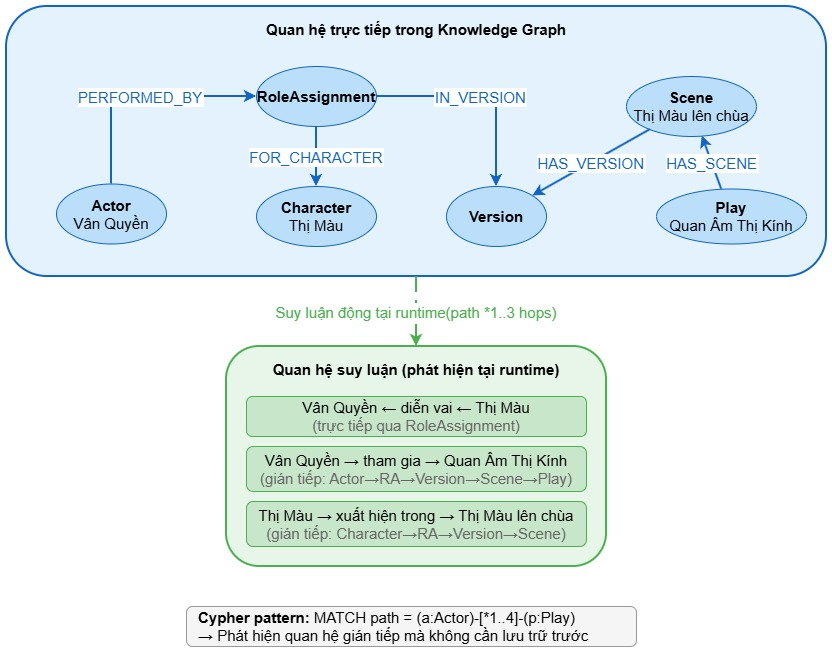
\includegraphics[width=\textwidth]{figures/c3/inference_rules.jpg}
  \caption{Ba chuỗi suy luận quan hệ gián tiếp của Chèo Knowledge Graph.}
  \label{fig:inference_rules}
\end{figure}

Toàn bộ suy luận được triển khai ở tầng ứng dụng --- không phụ thuộc vào OWL
reasoner --- nhờ đó duy trì độ trễ thấp và kiểm soát được phạm vi suy luận theo
từng loại câu hỏi.
% ============================================================

\subsection{Chiến lược lập chỉ mục tri thức}

Lược đồ được thiết kế ở các mục trước xác định \textit{cái gì} có trong đồ thị;
chiến lược lập chỉ mục xác định \textit{tốc độ} truy cập vào từng loại thông tin đó.
Ba tầng chỉ mục được thiết kế theo nguyên tắc khớp cơ chế lưu trữ với đặc điểm
phân bố của từng nhóm truy vấn, tổng hợp trong Bảng~\ref{tab:index_strategy}.

\begin{table}[ht]
  \centering
  \caption{Chiến lược chỉ mục ba tầng trên Chèo Knowledge Graph.}
  \label{tab:index_strategy}
  \renewcommand{\arraystretch}{1.35}
  \small
  \begin{tabular}{p{3.2cm} p{4.8cm} p{6.79cm}}
    \toprule
    \textbf{Tầng chỉ mục} & \textbf{Cơ chế Neo4j} & \textbf{Mục tiêu và truy vấn điển hình} \\
    \midrule
    Chỉ mục định danh
      & \texttt{UNIQUE} constraint trên thuộc tính \texttt{id} cho tất cả 7 loại nút gốc
      & Truy xuất $O(1)$ theo định danh chuẩn; đảm bảo tính idempotent khi nạp lại dữ liệu \\[4pt]
    Chỉ mục thuộc tính
      & B-tree index trên \texttt{charName}, \texttt{actorName}, \texttt{title}, \texttt{sceneName}
      & Tìm kiếm $O(\log n)$ theo tên thực thể - trường xuất hiện trong phần lớn câu hỏi người dùng \\[4pt]
    Chỉ mục toàn văn
      & \texttt{toLower()} + \texttt{CONTAINS} trên các trường tên
      & Khớp không phân biệt hoa/thường cho tên riêng tiếng Việt với nhiều biến thể viết tắt \\
    \bottomrule
  \end{tabular}
\end{table}

\textbf{Tầng~1 --- Chỉ mục định danh.}
Mỗi nút được gán \texttt{id} chuẩn duy nhất trong phạm vi nhãn của nó (ví dụ:
\texttt{play\_001}, \texttt{actor\_023}). Ràng buộc \texttt{UNIQUE} trên
\texttt{id} phục vụ đồng thời hai mục đích: (i)~truy xuất điểm đơn $O(1)$ khi
pipeline GraphRAG cần nạp một thực thể cụ thể từ kết quả suy luận, và
(ii)~đảm bảo tính idempotent cho phép \texttt{MERGE} trong quá trình nạp và
đồng bộ dữ liệu định kỳ.

\textbf{Tầng~2 --- Chỉ mục thuộc tính.}
Không có chỉ mục, cả SPARQL lẫn Cypher đều thực hiện full-scan toàn bộ nút khi
lọc theo tên --- chi phí $O(|V|)$ với mỗi truy vấn. B-tree index trên bốn trường
tên thường xuất hiện nhất (\texttt{charName}, \texttt{actorName}, \texttt{title},
\texttt{sceneName}) giảm chi phí xuống $O(\log|V|)$. Đây là tầng chỉ mục trực
tiếp giải quyết hạn chế~(3) của ontology gốc nêu ở Mục~3.2.1.

\textbf{Tầng~3 --- Chỉ mục toàn văn.}
Tên riêng tiếng Việt xuất hiện trong câu hỏi người dùng thường không đồng nhất
về cách viết hoa (``thị kính'', ``Thị Kính'', ``THỊ KÍNH''). Toàn bộ so sánh
chuỗi được chuẩn hóa qua \texttt{toLower()} trước khi áp dụng \texttt{CONTAINS},
đảm bảo truy vấn case-insensitive mà không cần lưu trữ bản sao thêm ---
giải quyết trực tiếp hạn chế~(4) từ Mục~3.2.1.

\begin{figure}[!ht]
  \centering
  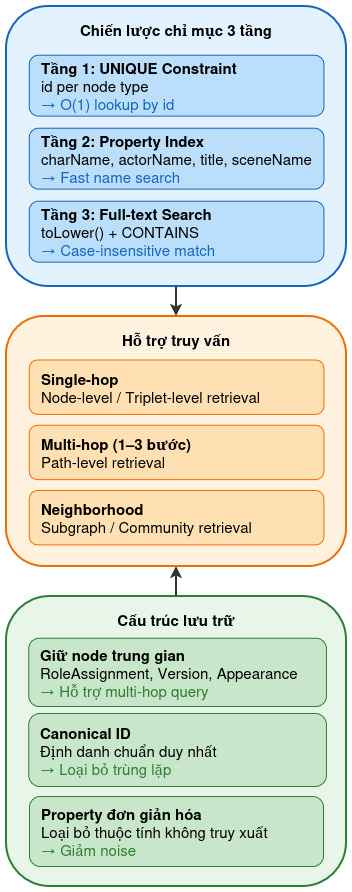
\includegraphics[width=0.5\textwidth]{figures/c3/indexing_data.jpg}
  \caption{Chiến lược chỉ mục ba tầng và vị trí áp dụng trên Chèo Knowledge Graph.}
  \label{fig:indexing_strategy}
\end{figure}

Ba tầng chỉ mục kết hợp bao phủ toàn bộ phổ truy vấn: tầng~1 phục vụ tra cứu
điểm đơn khi thực thể đã được định danh; tầng~2 phục vụ tìm kiếm theo tên trong
các câu hỏi trực tiếp; tầng~3 xử lý biến thể viết hoa trong đầu vào ngôn ngữ tự
nhiên. Cùng với lược đồ mở rộng (Mục~3.2.2) và suy luận động (Mục~3.2.3), ba
tầng chỉ mục hoàn thiện tầng tri thức của hệ thống GraphRAG.


\section{Thiết kế tầng xử lý GraphRAG}

\subsection{Thiết kế phân hệ G-Retrieval}

Phân hệ G-Retrieval chịu trách nhiệm xác định và trích xuất phần tri thức phù hợp từ Knowledge Graph để cung cấp ngữ cảnh cho quá trình tạo sinh câu trả lời. Trong kiến trúc GraphRAG, chất lượng câu trả lời phụ thuộc trực tiếp vào chất lượng ngữ cảnh được truy xuất; do đó, thiết kế của phân hệ này đóng vai trò quyết định đối với hiệu năng tổng thể của hệ thống.

Phân hệ G-Retrieval được tổ chức thành ba giai đoạn xử lý tuần tự (\textbf{Hình \ref{fig:g_retrieval_overview}}): (1) tiền xử lý và trích xuất thực thể, (2) truy vấn đa mức độ, và (3) tổ chức và lọc ngữ cảnh. Đầu vào tổng thể của phân hệ là câu hỏi ngôn ngữ tự nhiên $q$ từ người dùng; đầu ra là tập ngữ cảnh đã được định dạng  $C = \{(f_i, text_i)\}$, với $f_i$ là định dạng và $text_i$ là nội dung tương ứng, sẵn sàng để phân hệ G-Generation sử dụng.

\begin{figure}[!ht]
  \centering
  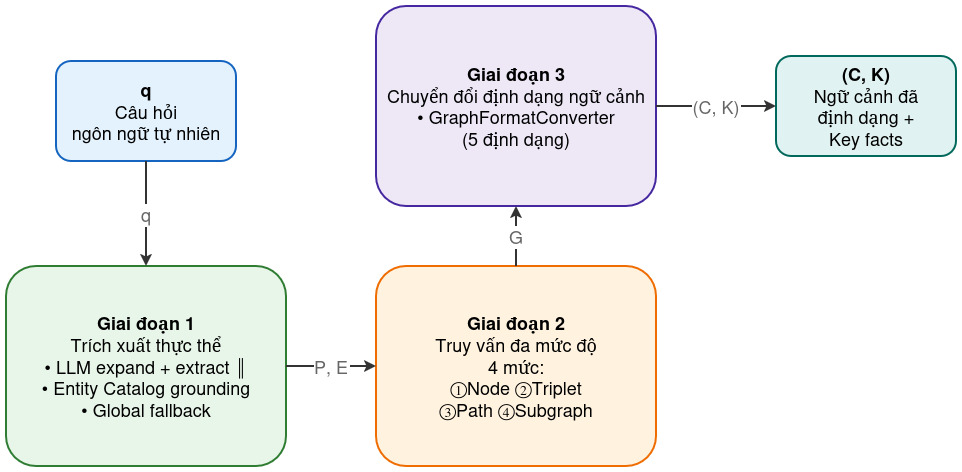
\includegraphics[width=\textwidth]{figures/c3/g_retrieval_overview.jpg}
  \caption{Sơ đồ tổng quan phân hệ G-Retrieval.}
  \label{fig:g_retrieval_overview}
\end{figure}


\subsubsection{Tiền xử lý và trích xuất thực thể}

Giai đoạn đầu tiên của phân hệ G-Retrieval thực hiện mở rộng truy vấn, phân rã câu hỏi và xác định các thực thể liên quan trong Knowledge Graph. Đây là bước thiết yếu vì các giai đoạn truy xuất tiếp theo phụ thuộc hoàn toàn vào tập thực thể được xác định tại bước này.

\textbf{Đầu vào.} Câu hỏi ngôn ngữ tự nhiên $q$ từ người dùng. Ví dụ:

\begin{tcolorbox}[colback=gray!5, colframe=black!50, arc=4pt, boxrule=0.5pt]
{\small
\begin{verbatim}
q = "Ai đóng vai Thị Màu trong vở Quan Âm Thị Kính?"
\end{verbatim}
}
\end{tcolorbox}

\textbf{Quy trình xử lý.} Hệ thống hỗ trợ hai chế độ xử lý: chế độ nâng cao (\textit{enhanced}, mặc định) và chế độ cơ bản (\textit{basic}) (\textbf{Hình \ref{fig:entity_extraction}}). Trong chế độ nâng cao, hệ thống sử dụng \texttt{ThreadPoolExecutor} để thực hiện đồng thời hai tác vụ LLM:

\begin{itemize}
  \item \textit{Luồng A (Mở rộng và trích xuất):} Gọi LLM với prompt \texttt{QUERY\_EXPAND \\ \_AND\_EXTRACT}, trong đó Entity Catalog --- danh mục chứa toàn bộ tên thực thể được nạp động từ Neo4j tại thời điểm khởi tạo hệ thống --- được đưa vào prompt làm tập tham chiếu. LLM trả về truy vấn mở rộng $q'$ và danh sách thực thể $E_{extracted}$ (các thực thể được chọn ra phải là các thực thể tồn tại trong Entity Catalog).
  \item \textit{Luồng B (Phân rã truy vấn):} Gọi LLM với prompt \texttt{QUERY\_DECOMPOSE} để phân rã câu hỏi gốc thành tập câu hỏi con $\{q_1, q_2, \ldots, q_n\}$.
\end{itemize}

Cơ chế song song hóa giảm độ trễ của giai đoạn tiền xử lý xuống xấp xỉ $\max(t_A, t_B)$ thay vì $t_A + t_B$ khi thực hiện tuần tự.

Trong chế độ cơ bản, truy vấn được sử dụng nguyên bản mà không qua mở rộng hay phân rã. Thực thể được trích xuất thông qua \texttt{EntityExtractor} với hai giai đoạn: (i)~trích xuất bằng biểu thức chính quy (\textit{regex}) cho danh từ riêng tiếng Việt, và (ii)~trích xuất bằng LLM qua prompt \texttt{ENTITY\_EXTRACT}. Kết quả từ cả hai giai đoạn được hợp nhất và loại bỏ trùng lặp.

\textbf{Đầu ra.} Sau khi trải qua quá trình phân tích và trích xuất, quy trình đưa ra hai đối tượng riêng biệt:
\begin{itemize}
  \item Đối tượng \texttt{ProcessedQuery} $P$ gồm ba thành phần: truy vấn gốc, truy vấn mở rộng và danh sách câu hỏi con.
  \item Tập thực thể $E$ phân loại theo bốn nhóm: \textit{characters}, \textit{actors}, \textit{plays}, \textit{scenes}.
\end{itemize}

\begin{tcolorbox}[colback=gray!5, colframe=black!50, arc=4pt, boxrule=0.5pt]
{\small
\begin{verbatim}
P = {
  original:   "Ai đóng vai Thị Màu
               trong vở Quan Âm Thị Kính?",
  expanded:   "Diễn viên nào đảm nhận vai diễn
               nhân vật Thị Màu trong vở chèo
               Quan Âm Thị Kính?",
  decomposed: [
    "Thị Màu là nhân vật trong vở nào?",
    "Ai đóng vai Thị Màu?"
  ]
}

E = {
  characters: ["Thị Màu"],
  actors: [],
  plays: ["Quan Âm Thị Kính"],
  scenes: []
}
\end{verbatim}
}
\end{tcolorbox}

\begin{figure}[!ht]
  \centering
  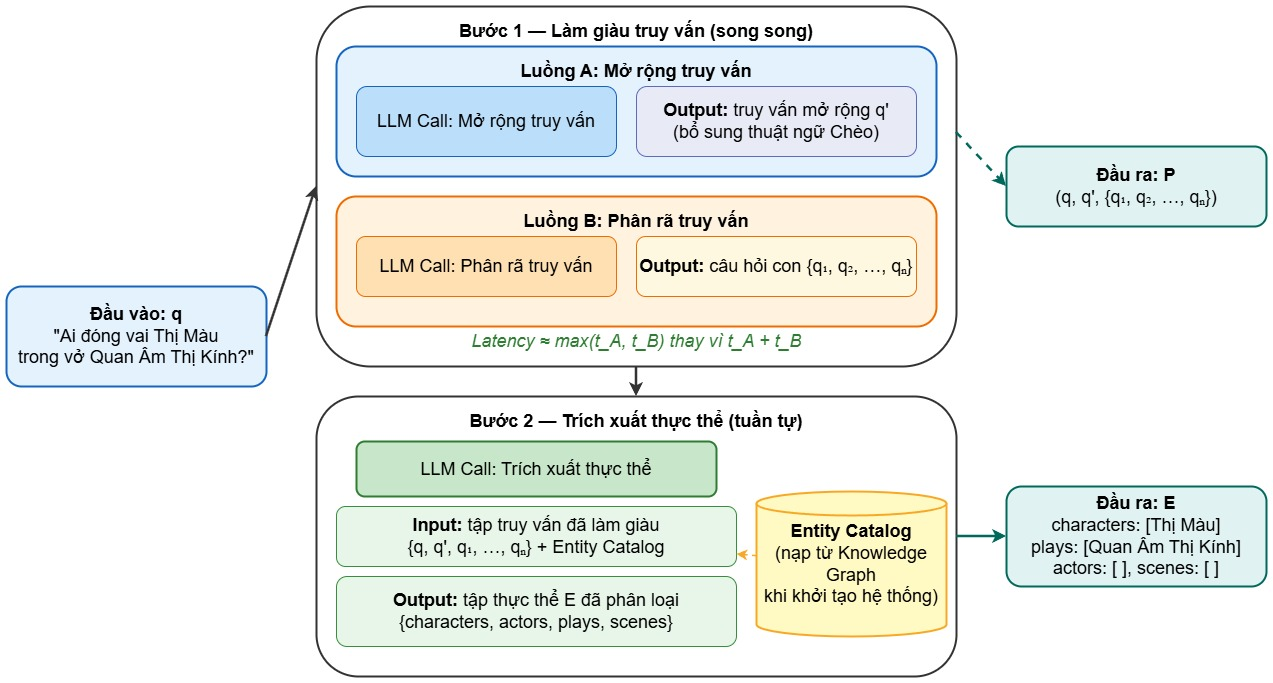
\includegraphics[width=\textwidth]{figures/c3/entity_extraction.jpg}
  \caption{Quy trình trích xuất thực thể song song.}
  \label{fig:entity_extraction}
\end{figure}


\subsubsection{Truy vấn đa mức độ}

Giai đoạn thứ hai thực hiện truy xuất tri thức từ Knowledge Graph dựa trên tập thực thể đã trích xuất $E$. Một câu hỏi đơn giản về nhân vật đòi hỏi loại thông tin hoàn toàn khác so với một câu hỏi so sánh xuyên suốt nhiều vở diễn. Chính vì thế nếu hệ thống sử dụng cùng một chiến lược truy xuất cho mọi loại truy vấn, câu trả lời sẽ bị thiếu thông tin (khi chiến lược quá nông, ít dữ liệu) hoặc chứa quá nhiều nhiễu (khi chiến lược quá rộng). Do đó, phân hệ G-Retrieval tổ chức \textbf{bốn mức độ truy xuất} (\textit{retrieval granularities}) (\textbf{Bảng~\ref{tab:retrieval_levels}}), mỗi mức khai thác một khía cạnh khác nhau của cấu trúc đồ thị, và lựa chọn tổ hợp mức phù hợp với độ phức tạp của từng loại truy vấn. Ngoài bốn mức truy xuất chính, hệ thống sử dụng \texttt{CommunityIndex} - một chỉ mục cộng đồng được xây dựng từ trước - nhằm cung cấp ngữ cảnh bổ sung cho các truy vấn ở mức độ cộng đồng và toàn cục.

\textbf{Đầu vào.} Tập thực thể $E$ từ giai đoạn tiền xử lý, cùng danh sách các mức truy xuất được kích hoạt (các mức này có thể là do con người chọn lựa, hoặc LLMs lựa chọn khi có danh sách các thực thể).

\begin{table}[ht]
  \centering
  \caption{Bốn mức độ truy vấn trong phân hệ G-Retrieval.}
  \label{tab:retrieval_levels}
  \resizebox{\textwidth}{!}{%
  \begin{tabular}{c l l l}
    \hline
    \textbf{Mức} & \textbf{Phương thức} & \textbf{Đầu ra} & \textbf{Vai trò} \\
    \hline
    \textcircled{1} Node & \texttt{MATCH (c:Label) WHERE ... CONTAINS} & Thuộc tính thực thể & Định danh, mô tả cơ bản \\
    \textcircled{2} Triplet & \texttt{MATCH (c)-[:FOR\_CHARACTER]-(ra)-[:PERFORMED\_BY]->(a)} & Bộ ba (S, P, O) & Quan hệ trực tiếp giữa 2 thực thể \\
    \textcircled{3} Path & \texttt{MATCH path = (start)-[*1..3]-(end)} & Chuỗi 1--3 bước & Suy luận đa bước qua trung gian \\
    \textcircled{4} Subgraph & \texttt{MATCH (center)-[*1..2]-(neighbor)} & Vùng lân cận 2-hop & Tổng hợp cấu trúc xung quanh thực thể \\
    \hline
  \end{tabular}%
  }
\end{table}

\textbf{Ánh xạ mức truy xuất theo loại truy vấn.} Mỗi loại truy vấn chỉ kích hoạt tập con các mức phù hợp, thay vì chạy đồng loạt tất cả gây tốn tài nguyên (\textbf{Bảng~\ref{tab:level_mapping}}).

\begin{table}[ht]
  \centering
  \caption{Ánh xạ mức truy xuất theo loại truy vấn.}
  \label{tab:level_mapping}
  \resizebox{\textwidth}{!}{%
  \begin{tabular}{l l l l}
    \hline
    \textbf{Loại truy vấn} & \textbf{Mức kích hoạt} & \textbf{Bổ trợ} & \textbf{Ví dụ} \\
    \hline
    Local & Node, Triplet & --- & ``Ai đóng vai Thị Màu?'' \\
    Community & Node, Triplet, Path & + CommunityIndex & ``Diễn viên nào đóng cả QATK lẫn Kim Nham?'' \\
    Global & Node, Triplet, Path, Subgraph & + CommunityIndex (global fallback) & ``So sánh số phận Súy Vân và Thị Kính'' \\
    \hline
  \end{tabular}%
  }
\end{table}

Với truy vấn \textbf{Local}, mức Node cung cấp thuộc tính thực thể (tên, giới tính, mô tả) và mức Triplet xác lập quan hệ trực tiếp (nhân vật--diễn viên, vở--nhân vật). Hai mức này đủ để trả lời các câu hỏi tra cứu đơn giản mà không sinh thêm ngữ cảnh dư thừa ảnh hưởng đến chất lượng prompt. Khi truy vấn thuộc cấp \textbf{Community}, hệ thống bổ sung mức Path để duyệt chuỗi quan hệ trung gian (ví dụ: Play $\rightarrow$ Character $\rightarrow$ RoleAssignment $\rightarrow$ Actor); đồng thời \texttt{CommunityIndex} cung cấp bối cảnh toàn bộ thực thể trong cùng cộng đồng vở, cho phép LLM thực hiện phép giao tập hợp hoặc so sánh nội hàm. Đối với truy vấn \textbf{Global}, tất cả bốn mức được kích hoạt: mức Subgraph mở rộng vùng lân cận xung quanh mỗi thực thể trung tâm với cấu trúc quan hệ đầy đủ, đồng thời \texttt{CommunityIndex} giúp bổ sung ngữ cảnh từ tất cả các vở, cung cấp nền tảng cho quá trình tổng hợp và phân tích xuyên suốt Knowledge Graph.

Mức \textbf{Node} thực hiện bốn truy vấn Cypher, mỗi truy vấn cho một nhãn thực thể (Character, Actor, Play, Scene), sử dụng phép so khớp \texttt{CONTAINS} không phân biệt hoa thường. Tất cả tên thực thể trong $E$ được gộp vào cùng một truy vấn thông qua mệnh đề \texttt{any(n IN \$names WHERE ...)}, giảm số lượt gọi Neo4j xuống đúng bốn lần bất kể số lượng thực thể. Giới hạn kết quả: 50 node mỗi nhãn. Khi không có kết quả khớp trực tiếp, mức này kích hoạt cơ chế dự phòng (\textit{fallback}): tìm kiếm mờ trên tất cả các thuộc tính với giới hạn 10 kết quả.

Mức \textbf{Triplet} sử dụng ba truy vấn riêng biệt cho ba mẫu quan hệ chính trong ontology Chèo: (i)~Character $\leftrightarrow$ Actor thông qua RoleAssignment --- truy vấn quan trọng nhất, liên kết nhân vật với diễn viên; (ii)~Play $\rightarrow$ Character qua quan hệ \texttt{HAS\_CHARACTER}; và (iii)~Play $\rightarrow$ Scene qua quan hệ \texttt{HAS\_SCENE}. Mỗi truy vấn trả về bộ ba $(S, P, O)$ và giới hạn tại 50 triplet. Khi không có kết quả, mức Triplet trả về một mẫu quan hệ diễn viên--nhân vật tiêu biểu làm dự phòng.

Mức \textbf{Path} thực hiện một truy vấn duyệt đường dẫn biến đổi trong đồ thị: \texttt{MATCH path = (start)-[*1..3]-(end)}, trong đó điểm bắt đầu là các thực thể thuộc nhóm Character, Actor hoặc Play trong $E$. Hệ thống trích xuất tên hiển thị của tất cả node trên đường dẫn qua hàm \texttt{coalesce()}, tạo ra chuỗi dạng ``Thị Màu $\rightarrow$ RA\_042 $\rightarrow$ Version\_01 $\rightarrow$ Trích đoạn: ...'' giúp LLM nhận diện chuỗi suy luận trung gian. Số hop tối đa là 3 và giới hạn là 30 đường dẫn. Mức này đặc biệt hữu ích cho truy vấn Community, nơi câu trả lời nằm cách thực thể gốc nhiều bước nhảy.

Mức \textbf{Subgraph} mở rộng vùng lân cận xung quanh mỗi thực thể trung tâm: \texttt{MATCH path = (center)-[*1..2]-(neighbor)}, sau đó thu thập cả node lẫn relationship trên các đường dẫn. Khác với mức Path chỉ trả về chuỗi tên, mức Subgraph trả về cấu trúc đồ thị đầy đủ gồm thuộc tính node và kiểu quan hệ, được biểu diễn dưới dạng \texttt{\{nodes: [...], relationships: [\{type, start, end\}]\}}. Giới hạn là 10 mở rộng, tối đa 2 hop. Mức này cung cấp ngữ cảnh phong phú nhất cho truy vấn Global, nơi LLM cần hiểu cấu trúc quan hệ tổng thể xung quanh thực thể để tổng hợp và so sánh.

\textbf{Chỉ mục cộng đồng (CommunityIndex).} Bên cạnh bốn mức truy xuất trực tiếp từ Neo4j, hệ thống sử dụng \texttt{CommunityIndex} --- một chỉ mục tri thức được tiền xây dựng tại thời điểm khởi tạo thông qua ba truy vấn Cypher nhóm theo Play node:
\begin{itemize}
  \item \texttt{Play} $\xrightarrow{\text{HAS\_CHARACTER}}$ \texttt{Character}: nhân vật thuộc vở.
  \item \texttt{Play} $\xrightarrow{\text{HAS\_SCENE}}$ \texttt{Scene}: trích đoạn thuộc vở.
  \item Đường dẫn \texttt{RoleAssignment} $\rightarrow$ \texttt{Actor}, \texttt{Character}, \texttt{Version}, \texttt{Scene} $\rightarrow$ \texttt{Play}: thông tin đầy đủ của các vai diễn.
\end{itemize}

\textbf{Đầu ra.} Đối tượng \texttt{GraphData} $G$ (\textbf{Hình \ref{fig:multi_granularity}})chứa kết quả từ các mức được kích hoạt, bổ sung bởi ngữ cảnh từ CommunityIndex:

\begin{tcolorbox}[colback=gray!5, colframe=black!50, arc=4pt, boxrule=0.5pt]
{\small
\begin{verbatim}
G = {
  nodes:    [{charName: "Thị Màu", ...}, ...],
  triplets: [("Thị Màu", "PERFORMED_BY",
              "Vân Quyền"), ...],
  paths:    [["Thị Màu", "RA_042",
              "Version_01", "Scene:..."], ...],
  subgraph: {nodes: [...],
             relationships: [...]},
  community_context: "=== Quan Âm Thị Kính ===
    Nhân vật (15): Thị Màu, Thị Kính, ...
    Diễn viên (8): Vân Quyền, Ấn Chính, ..."
}
\end{verbatim}
}
\end{tcolorbox}

Tùy loại truy vấn, một số key trong \texttt{GraphData} có thể rỗng: truy vấn Local thường chỉ có \texttt{nodes} và \texttt{triplets} chứa dữ liệu, trong khi \texttt{paths}, \texttt{subgraph} và \texttt{community\_context} trống. Điều này giúp kiểm soát kích thước ngữ cảnh gửi đến LLM, tránh hiện tượng pha loãng thông tin quan trọng bởi dữ liệu không liên quan.

\begin{figure}[!ht]
  \centering
  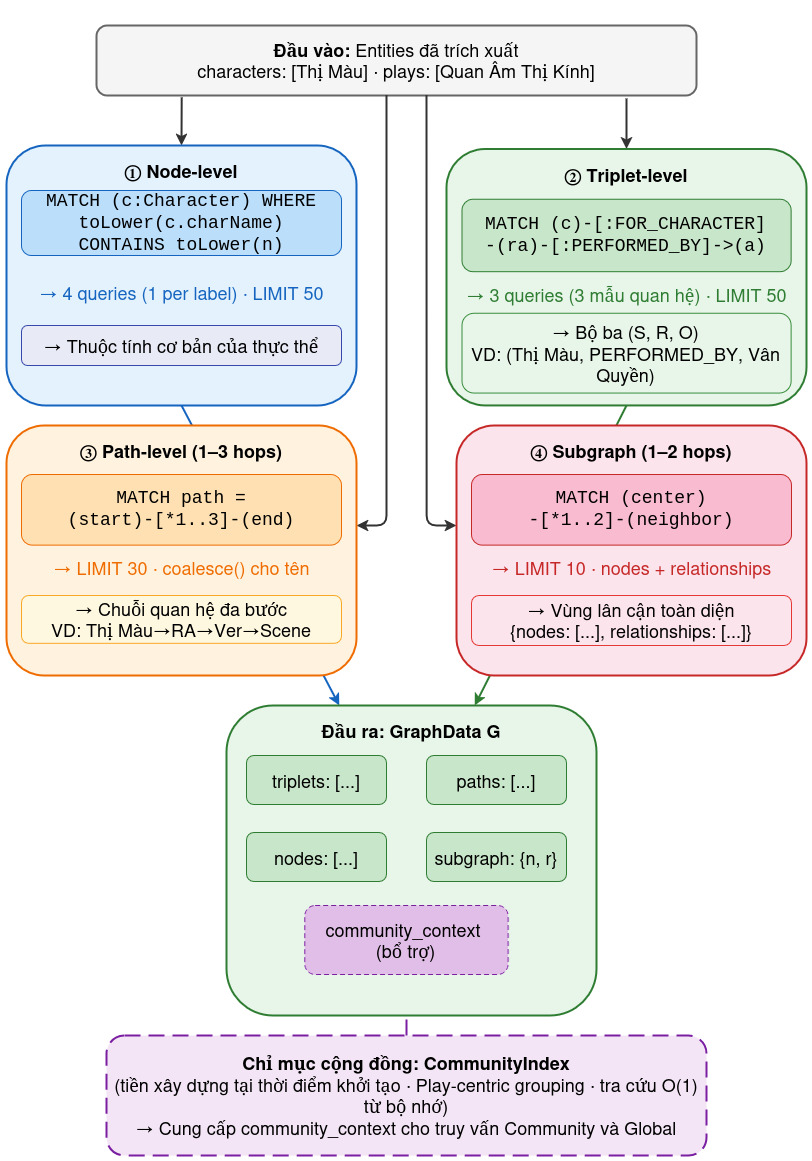
\includegraphics[width=\textwidth]{figures/c3/multi_granularity.jpg}
  \caption{Bốn mức truy vấn đa mức độ và chỉ mục cộng đồng CommunityIndex.}
  \label{fig:multi_granularity}
\end{figure}


\subsubsection{Tổ chức ngữ cảnh}

Giai đoạn cuối cùng của phân hệ G-Retrieval thực hiện chuyển đổi dữ liệu đồ thị thô thành các biểu diễn văn bản phù hợp với mô hình ngôn ngữ.

\textbf{Đầu vào.} Đối tượng \texttt{GraphData} $G$ từ giai đoạn truy xuất.

\textbf{Quy trình xử lý.} Khác với văn bản tuần tự, \texttt{GraphData} $G$ cung cấp thông tin ở nhiều mức độ khác nhau, do đó mỗi cách biểu diễn cung cấp một nguồn tri thức phù hợp với tác vụ được yêu cầu (\textbf{Hình \ref{fig:context_organization}}) . Lớp \texttt{GraphFormatConverter} trực tiếp xử lý dữ liệu đồ thị được tiếp nhận (\textbf{Bảng~\ref{tab:format_converter}}), chuyển hóa thành năm định dạng văn bản riêng biệt. Quá trình này cung cấp các góc nhìn đa chiều về tri thức để hỗ trợ mô hình ngôn ngữ suy luận. Việc ứng dụng các định dạng thông tin này dựa trên chiến lược tạo sinh sẽ được trình bày chi tiết trong phần tiếp theo. 

\begin{table}[ht]
  \centering
  \caption{Năm định dạng chuyển hóa thông tin}
  \label{tab:format_converter}
  \resizebox{\textwidth}{!}{%
  \begin{tabular}{l l p{8cm}}
    \hline
    \textbf{Định dạng} & \textbf{Phương thức} & \textbf{Giá trị cốt lõi} \\
    \hline
    natural\_language & \texttt{to\_natural\_language()} & Khai thác năng lực hiểu ngôn ngữ của LLM, văn phong tự nhiên \\
    adjacency\_table & \texttt{to\_adjacency\_table()} & Cung cấp cấu trúc lưới chéo, hạn chế ảo giác (hallucination) \\
    code\_like & \texttt{to\_code\_like()} & Bảo toàn tuyệt đối schema và siêu dữ liệu (metadata) qua JSON \\
    node\_sequence & \texttt{to\_node\_sequence()} & Trực quan hóa các ràng buộc liên kết đa bước (multi-hop) \\
    community\_summary & \texttt{to\_community\_summary()} & Cung cấp tổng quan thông tin trong đồ thị tri thức \\
    \hline
  \end{tabular}%
  }
\end{table}

\textbf{Định dạng ngôn ngữ tự nhiên (\texttt{natural\_language}).} Định dạng này thực hiện chuyển đổi trực tiếp các cấu trúc bộ ba (triplet) thành câu văn tiếng Việt hoàn chỉnh thông qua bảng ánh xạ từ vựng \texttt{\_REL\_VERB} (ví dụ: quan hệ \texttt{HAS\_CHARACTER} thành ``có nhân vật''). Phương pháp biểu diễn này có khả năng kết hợp linh hoạt với dữ liệu thu được từ hai mức độ truy xuất \textit{Node} và \textit{Triplet}. Các biểu diễn này tận dụng khả năng xử lý và suy luận văn bản vốn có của mô hình ngôn ngữ lớn (LLM), bằng cách cung cấp một luồng lý luận bằng ngôn ngữ chuẩn mực giúp kết quả mô hình sinh ra mang văn phong tự nhiên, sát thực với đặc thù giao tiếp của miền dữ liệu nghệ thuật Chèo.

\vspace{0.5em}
\begin{tcolorbox}[colback=gray!5, colframe=black!50, arc=4pt, boxrule=0.5pt, left=4pt, right=4pt, top=4pt, bottom=4pt, boxsep=0pt]
\small \texttt{"Nhân vật Thị Màu thuộc vở diễn Quan Âm Thị Kính và được thể hiện bởi diễn viên Vân Quyền."}
\end{tcolorbox}

\textbf{Định dạng bảng kề Markdown (\texttt{adjacency\_table}).} Cấu trúc đồ thị được triết xuất thành một bảng hai chiều nghiêm ngặt gồm ba cột: Nút Khởi Đầu, Quan Hệ và Nút Đích. Định dạng này phát huy tối đa hiệu quả khi xử lý dữ liệu từ mức độ \textit{Triplet}. Cấu trúc dạng lưới chéo tạo ranh giới dữ liệu phân minh, giúp mô hình ngôn ngữ dễ dàng thao tác đối chiếu (cross-reference) thông tin, đồng thời giảm nguy cơ loãng thông tin khi gặp các cấu trúc văn bản có mật độ cao. Từ đó, mô hình kiểm soát chặt chẽ hiện tượng ảo giác (hallucination) khi truy vấn các hệ thực thể đan xen phức tạp.

\vspace{0.5em}
\begin{tcolorbox}[colback=gray!5, colframe=black!50, arc=4pt, boxrule=0.5pt, left=4pt, right=4pt, top=4pt, bottom=4pt, boxsep=0pt]
\small
\begin{verbatim}
| Nút Khởi Đầu | Loại Quan Hệ | Nút Đích         |
|--------------|--------------|------------------|
| Thị Màu      | THUỘC_VỞ     | Quan Âm Thị Kính |
| Thị Màu      | ĐÓNG_BỞI     | Vân Quyền        |
\end{verbatim}
\end{tcolorbox}

\textbf{Định dạng cấu trúc JSON (\texttt{code\_like}).} Trong biểu diễn này, toàn bộ mạng lưới các nút cùng hệ siêu dữ liệu (metadata) tương ứng được đóng gói thành các đối tượng JSON. Đây là phương pháp biểu diễn tối ưu nhất để tiếp nhận nguyên vẹn lượng dữ liệu phức tạp từ chiều sâu của mức độ \textit{Subgraph}. Việc bảo toàn hệ phân loại (taxonomy) của Knowledge Graph cho phép LLM duy trì tư duy phân tích hệ thống, hiệu quả hơn trong việc thực thi các truy vấn mang tính cấu trúc hình học hoặc bóc tách tham số chi tiết của nhiều đối tượng liên kết dày đặc.

\vspace{0.5em}
\begin{tcolorbox}[colback=gray!5, colframe=black!50, arc=4pt, boxrule=0.5pt, left=4pt, right=4pt, top=4pt, bottom=4pt, boxsep=0pt]
\small
\begin{verbatim}
{
  "nodes": [{"id": "Thị Màu", "label": "Character"}],
  "relationships": [{"start": "Thị Màu", "type": "THUỘC_VỞ",
                     "end": "Quan Âm Thị Kính"}]
}
\end{verbatim}
\end{tcolorbox}

\textbf{Định dạng chuỗi thực thể (\texttt{node\_sequence}).} Biểu diễn này tái định hình sự phụ thuộc không gian của đồ thị thành chuỗi tuyến tính trực quan dưới dạng $A \rightarrow B \rightarrow C$. Định dạng chuỗi thực thể được thiết kế kế thừa trực tiếp kết quả của mức độ \textit{Path}, mô phỏng các tuyến đường dẫn đa bước (multi-hop). Cách tiếp cận này cung cấp một lộ trình suy diễn có sẵn, thúc đẩy trực tiếp hiệu suất cho các câu hỏi mang tính diễn biến tuần tự hoặc truy tìm nguồn gốc nhiều tầng.

\vspace{0.5em}
\begin{tcolorbox}[colback=gray!5, colframe=black!50, arc=4pt, boxrule=0.5pt, left=4pt, right=4pt, top=4pt, bottom=4pt, boxsep=0pt]
\small \texttt{Vân Quyền $\rightarrow$ Thị Màu $\rightarrow$ Quan Âm Thị Kính}
\end{tcolorbox}

\textbf{Định dạng tóm tắt cộng đồng (\texttt{community\_summary}).} Định dạng này đảm nhiệm vai trò hệ thống hóa thông tin \texttt{community\_context} được trích xuất từ \textit{CommunityIndex}, cung cấp các chỉ số thống kê quy mô và danh sách phân rã thực thể theo từng cụm thông tin trong đồ thị tri thức (như cụm Vở diễn). Tóm tắt cộng đồng cung cấp cho LLM cái nhìn toàn cảnh về cấu trúc tổ chức của các thực thể, từ đó tạo nền tảng ngữ cảnh cho LLMs xử lý chuẩn xác các tình huống truy vấn toàn cục (Global query) mà không bị thất thoát thông tin tổng thể.

\vspace{0.5em}
\begin{tcolorbox}[colback=gray!5, colframe=black!50, arc=4pt, boxrule=0.5pt, left=4pt, right=4pt, top=4pt, bottom=4pt, boxsep=0pt]
\small
\begin{verbatim}
=== Vở Quan Âm Thị Kính ===
- Số lượng: 15 nhân vật, 8 diễn viên
- Danh sách nhân vật: Thị Màu, Thị Kính, Thiện Sĩ, ...
- Danh sách diễn viên: Vân Quyền, Thu Huyền, ...
\end{verbatim}
\end{tcolorbox}

\textbf{Đầu ra.} Hai thành phần:
\begin{itemize}
  \item Tập ngữ cảnh đa định dạng $C = \{(f_i, text_i)\}$ với $f_i$ là định dạng và $text_i$ là nội dung tương ứng.
  \item Tập dữ kiện chính $K$ (\textit{key facts}) dạng bullet points tóm tắt thông tin quan trọng nhất, được trích xuất bởi \texttt{extract\_key\_facts()} từ dữ liệu đồ thị.
\end{itemize}

\begin{figure}[!ht]
  \centering
  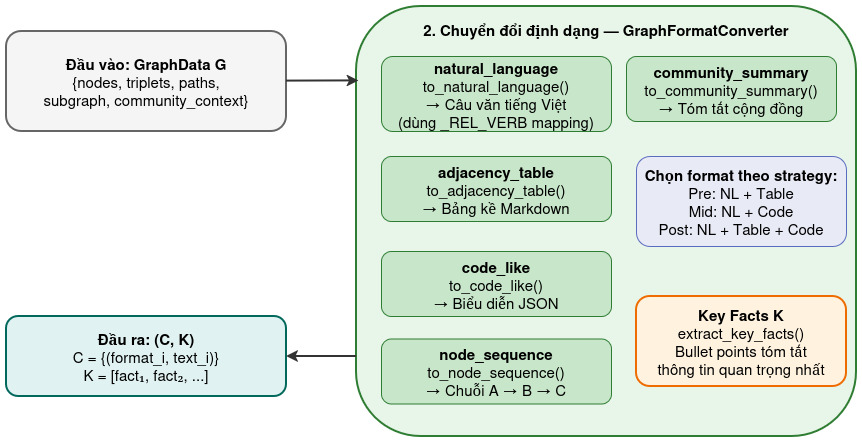
\includegraphics[width=\textwidth]{figures/c3/context_organization.jpg}
  \caption{Quy trình tổ chức ngữ cảnh.}
  \label{fig:context_organization}
\end{figure}
% ===========================================================
\subsection{Thiết kế phân hệ G-Generation}

Phân hệ G-Generation chịu trách nhiệm chuyển hóa ngữ cảnh tri thức đồ thị đã được định dạng từ phân hệ G-Retrieval thành câu trả lời ngôn ngữ tự nhiên thông qua các mô hình ngôn ngữ lớn (LLMs). Với kiến trúc phân tầng, LLMs không truy cập trực tiếp Knowledge Graph mà chỉ tiếp nhận ngữ cảnh văn bản đã qua xử lý và định dạng bởi giai đoạn G-Retrieval. Cách tiếp cận này mang lại hai ưu thế quan trọng --- khả năng thay thế LLMs mà không ảnh hưởng đến pipeline truy xuất, và khả năng kiểm soát chặt chẽ lượng thông tin mà mô hình nhận được.

Về mặt kiến trúc, phân hệ G-Generation được cấu thành từ hai thành phần chính: lớp điều phối \texttt{GenerationOrchestrator} và hệ thống chiến lược tạo sinh (\texttt{BaseGenerationStrategy}). Đầu vào tổng thể là bộ $(C, K, q)$ --- trong đó $C = \{(f_i, text_i)\}$ là tập ngữ cảnh đa định dạng, $K$ là tập dữ kiện chính, và $q$ là câu hỏi gốc --- kế thừa trực tiếp từ đầu ra của giai đoạn Tổ chức ngữ cảnh. Đầu ra là câu trả lời dưới dạng ngôn ngữ tự nhiên $a$(\textbf{Hình~\ref{fig:g_generation_overview}}).

\begin{figure}[!ht]
  \centering
  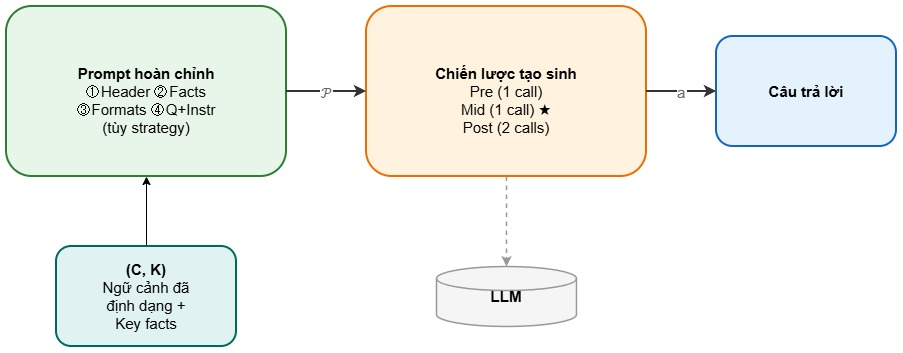
\includegraphics[width=\textwidth]{figures/c3/g_generation_overview.jpg}
  \caption{Sơ đồ tổng quan phân hệ G-Generation.}
  \label{fig:g_generation_overview}
\end{figure}


\subsubsection{Xây dựng cấu trúc Prompt}

LLM được sử dụng trong hệ thống không trải qua quá trình huấn luyện bổ sung (\textit{fine-tuning}) cho miền dữ liệu nghệ thuật Chèo. Toàn bộ tri thức miền được cung cấp thông qua cơ chế tiêm ngữ cảnh tại thời điểm suy luận (\textit{inference-time context injection}): tập ngữ cảnh đa định dạng $C$ và dữ kiện chính $K$ --- đã được giai đoạn Tổ chức ngữ cảnh của G-Retrieval chuẩn bị hoàn chỉnh --- được tổ hợp thành chuỗi văn bản liền mạch rồi ghép vào prompt gửi đến LLM.

Chuỗi ngữ cảnh đã tổ hợp $\mathcal{C}$ sau đó được ghép với câu hỏi $q$ và chỉ dẫn tạo sinh theo một cấu trúc prompt cố định gồm bốn thành phần tuần tự, như trình bày trong Bảng~\ref{tab:prompt_structure}. Nguyên tắc then chốt là đặt toàn bộ tri thức hỗ trợ (①②③) trước câu hỏi (④), phù hợp với cơ chế phân bổ trọng số chú ý (attention weight distribution) của kiến trúc Transformer --- mô hình có xu hướng tham chiếu mạnh hơn tới các token xuất hiện trước trong chuỗi đầu vào khi thực hiện suy luận.

\begin{table}[ht]
  \centering
  \caption{Các thành phần cấu trúc prompt.}
  \label{tab:prompt_structure}
  \resizebox{\textwidth}{!}{%
  \begin{tabular}{c l l l}
    \hline
    \textbf{TT} & \textbf{Thành phần} & \textbf{Nội dung} & \textbf{Nguồn} \\
    \hline
    \textcircled{1} & Context Header & ``Thông tin từ Knowledge Graph về Chèo'' & Hằng số cố định \\
    \textcircled{2} & Key Facts & Tóm tắt dữ kiện quan trọng (bullet points) & $K$ từ G-Retrieval \\
    \textcircled{3} & Format Sections & Ngữ cảnh theo các định dạng được chọn & $C$ từ G-Retrieval \\
    \textcircled{4} & Câu hỏi + Chỉ dẫn & Câu hỏi và ràng buộc tạo sinh & Template theo strategy \\
    \hline
  \end{tabular}%
  }
\end{table}

Việc lựa chọn tập con định dạng nào trong $C$ để đưa vào prompt phụ thuộc vào đặc tính của câu hỏi và chiến lược tạo sinh, không phải là phép gán cứng. Năm định dạng từ giai đoạn Tổ chức ngữ cảnh có mức độ tương thích tự nhiên khác nhau với từng chiến lược:
\begin{itemize}
  \item \texttt{natural\_language} có tính phổ quát cao, phù hợp với mọi chiến lược vì tận dụng trực tiếp năng lực đọc hiểu văn bản vốn có của LLM.
  \item \texttt{adjacency\_table} phát huy tối đa hiệu quả khi chiến lược cần đối chiếu chéo nhiều quan hệ (Pre, Post), nhờ cấu trúc bảng phân tách rõ ràng ranh giới thực thể.
  \item \texttt{code\_like} (JSON) thích hợp với các chiến lược yêu cầu bóc tách siêu dữ liệu chi tiết (Mid, Post), đặc biệt khi câu hỏi đòi hỏi phân tích thuộc tính từ mức Subgraph.
  \item \texttt{node\_sequence} hữu ích khi câu hỏi mang tính truy vết nhiều bước (multi-hop), cung cấp sẵn lộ trình suy diễn tuyến tính cho LLM.
  \item \texttt{community\_summary} được kích hoạt chủ yếu cho các truy vấn toàn cục (Global), cung cấp bức tranh vĩ mô về phân bố thực thể theo cụm cộng đồng.
\end{itemize}

Việc kiểm soát độ dài ngữ cảnh tổng thể được đảm bảo bởi mệnh đề \texttt{LIMIT} trong truy vấn Cypher ở tầng G-Retrieval --- giới hạn lượng dữ liệu thô ngay từ nguồn. Số lượng định dạng kích hoạt trong prompt cũng ảnh hưởng trực tiếp: các chiến lược đơn giản (Pre) có xu hướng sử dụng ít định dạng hơn (2 formats) để tối ưu tốc độ, trong khi chiến lược phức tạp (Post) có thể khai thác nhiều định dạng hơn (3+ formats) nhờ cơ chế đối chiếu hai lượt bù đắp chi phí.

Ví dụ một prompt $\mathcal{P}$ hoàn chỉnh (chiến lược Pre) cho câu hỏi ``Ai đóng vai Thị Màu?'':

\begin{tcolorbox}[colback=gray!5, colframe=black!50, arc=4pt, boxrule=0.5pt, left=4pt, right=4pt, top=4pt, bottom=4pt]
{\small
\begin{verbatim}
# Thông tin từ Knowledge Graph về Chèo      ← ①

## Tóm tắt quan trọng:                      ← ②
- Nhân vật: Thị Màu
- Diễn viên: Vân Quyền
- Vở: Quan Âm Thị Kính

## Mô tả tự nhiên:                          ← ③
Nhân vật Thị Màu thuộc vở diễn Quan Âm
Thị Kính và được thể hiện bởi Vân Quyền.

## Bảng quan hệ:                            ← ③
| Nút Bắt Đầu | Quan Hệ    | Nút Đích         |
|-------------|------------|-------------------|
| Thị Màu     | THUỘC_VỞ   | Quan Âm Thị Kính  |
| Thị Màu     | ĐÓNG_BỞI   | Vân Quyền         |

# Câu hỏi                                  ← ④
Ai đóng vai Thị Màu?

# Yêu cầu
Trả lời dựa trên thông tin graph ở trên.
Nhớ cite cụ thể tên từ graph.
\end{verbatim}
}
\end{tcolorbox}

\begin{figure}[ht]
  \centering
  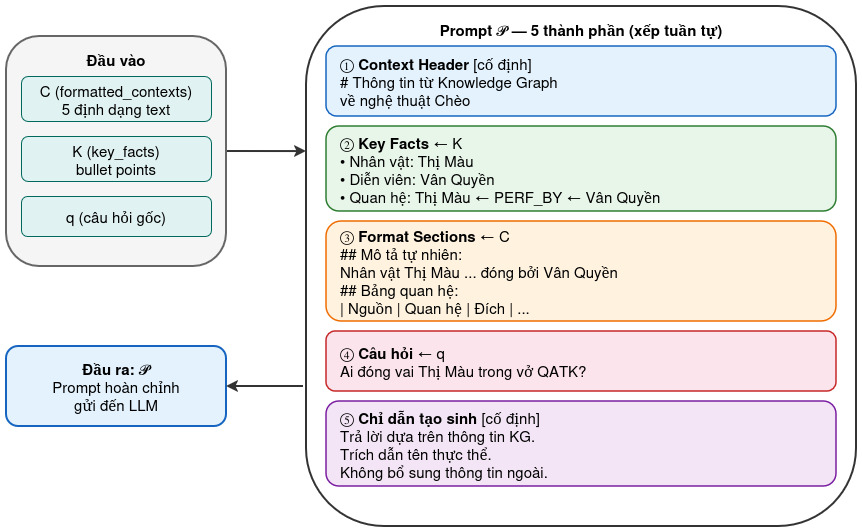
\includegraphics[width=0.85\textwidth]{figures/c3/prompt_structure.jpg}
  \caption{Cấu trúc các thành phần của prompt.}
  \label{fig:prompt_structure}
\end{figure}


\subsubsection{Các chiến lược tạo sinh}

Phân hệ G-Generation triển khai ba chiến lược tạo sinh (\textbf{Hình \ref{fig:generation_strategies}}), kế thừa từ lớp trừu tượng \texttt{BaseGenerationStrategy}. Mỗi chiến lược có một nhiệm vụ khác nhau, cân bằng giữa độ chính xác, chi phí tính toán và số lượt gọi LLMs.

Chiến lược \textbf{Pre-Generation} tiếp cận bài toán tạo sinh theo hướng tối ưu hóa biểu diễn đầu vào, trong đó toàn bộ ngữ cảnh truy xuất được từ Knowledge Graph được tổ chức và cung cấp trực tiếp cho mô hình dưới dạng một prompt duy nhất. Trong thiết kế này, mô hình ngôn ngữ được xem như một bộ suy luận dạng hộp đen, không bị ràng buộc bởi bất kỳ cấu trúc suy luận tường minh nào. Do đó, hiệu quả của chiến lược phụ thuộc chủ yếu vào chất lượng và mức độ rõ ràng của ngữ cảnh đầu vào. Giá trị cốt lõi của Pre-Generation nằm ở khả năng khai thác tối đa năng lực suy luận nội tại của LLM với chi phí thấp và độ trễ nhỏ, đặc biệt phù hợp với các truy vấn tra cứu trực tiếp, nơi mối quan hệ giữa thực thể đã được biểu diễn rõ ràng trong dữ liệu.

Chiến lược \textbf{Mid-Generation} tập trung vào việc kiểm soát quá trình suy luận của mô hình thông qua việc áp đặt một khuôn mẫu tạo sinh có cấu trúc. Thay vì để mô hình tự do tổng hợp câu trả lời, prompt được thiết kế để buộc LLM thực hiện tuần tự các bước trích xuất dữ kiện, phân tích và kết luận. Cách tiếp cận này chuyển vai trò của mô hình từ một bộ sinh ngôn ngữ thuần túy sang một hệ thống suy luận có kiểm soát, trong đó mọi kết luận đều phải được liên kết rõ ràng với bằng chứng từ ngữ cảnh. So với Pre-Generation, Mid-Generation đánh đổi một phần chi phí để đạt được độ tin cậy cao hơn, đặc biệt trong các truy vấn yêu cầu suy luận nhiều bước hoặc tổng hợp thông tin từ nhiều quan hệ trong đồ thị.

Chiến lược \textbf{Post-Generation} mở rộng thêm một bước kiểm định hậu kỳ nhằm xử lý các sai lệch tiềm ẩn trong quá trình tạo sinh. Cụ thể, mô hình trước tiên sinh ra một câu trả lời sơ bộ dựa trên tri thức tham số hóa, sau đó câu trả lời này được đối chiếu với ngữ cảnh từ Knowledge Graph để phát hiện và hiệu chỉnh sai sót. Cách tiếp cận hai bước này cho phép tách biệt rõ ràng giữa quá trình sinh và quá trình kiểm chứng, qua đó phát hiện được sự không nhất quán giữa tri thức nội tại của mô hình và dữ liệu thực tế. Giá trị chính của Post-Generation nằm ở khả năng nâng cao độ chính xác và độ tin cậy của đầu ra, đặc biệt trong các truy vấn phức tạp hoặc yêu cầu tính chính xác cao, mặc dù phải đánh đổi bằng chi phí tính toán và độ trễ lớn hơn.

\textbf{Đầu vào.} Prompt $\mathcal{P}$ đã tổ hợp từ giai đoạn trước.

\textbf{Quy trình xử lý.} \texttt{GenerationOrchestrator} xác định chiến lược tạo sinh, tổng hợp thông tin và thực hiện gọi LLMs để cung cấp cho người dùng câu trả lời cuối cùng dưới dạng ngôn ngữ tự nhiên.

\textbf{Đầu vào.} Cuối của quá trình này, một câu trả lời ngôn ngữ tự nhiên đã cơ bản được hoàn thành, sẵn sàng cho việc hiển thị tới người dùng.

\vspace{0.5em}
\noindent \textit{Ví dụ đầu ra chiến lược Mid} (câu hỏi: ``Ai đóng vai Thị Màu?''):
\begin{tcolorbox}[colback=gray!5, colframe=black!50, arc=4pt, boxrule=0.5pt]
{\small
\begin{verbatim}
1. Thông tin từ graph:
   - Nhân vật: Thị Màu
   - Diễn viên: Vân Quyền
   - Quan hệ: Thị Màu ← PERFORMED_BY ← Vân Quyền

2. Phân tích:
   Theo dữ liệu Knowledge Graph, nhân vật Thị Màu
   được thể hiện bởi diễn viên Vân Quyền.

3. Kết luận:
   Vai Thị Màu được đóng bởi Vân Quyền.
\end{verbatim}
}
\end{tcolorbox}



\vspace{0.5em}
\noindent \textit{Ví dụ luồng xử lý chiến lược Post}:
\begin{tcolorbox}[colback=gray!5, colframe=black!50, arc=4pt, boxrule=0.5pt]
{\small
\begin{verbatim}
Lượt 1: sinh câu trả lời sơ bộ (không có context)
→ kết quả mơ hồ

Lượt 2: đối chiếu với graph + key facts
→ sửa và tạo câu trả lời chính xác
\end{verbatim}
}
\end{tcolorbox}

Tổng thể, phần quan trọng nhất trong quá trình này chính là ba chiến lược tạo sinh. Chúng không tồn tại độc lập mà hình thành một phổ liên tục về mức độ kiểm soát đối với quá trình suy luận của mô hình. Chiến lược Pre-Generation ưu tiên tối ưu hóa đầu vào và tận dụng năng lực suy luận nội tại của LLM với chi phí thấp, trong khi Mid-Generation bổ sung các ràng buộc cấu trúc nhằm định hướng quá trình suy luận và nâng cao độ tin cậy của kết quả. Ở mức cao nhất, Post-Generation triển khai thêm cơ chế kiểm định hậu kỳ để phát hiện và hiệu chỉnh sai lệch, qua đó đạt được độ chính xác tối ưu nhưng đánh đổi bằng chi phí và độ trễ lớn hơn. Sự khác biệt này được tổng hợp một cách hệ thống trong Bảng~\ref{tab:gen_strategies}, cho thấy rõ mối quan hệ đánh đổi giữa số lượt gọi mô hình, mức độ kiểm soát suy luận và chất lượng đầu ra. Thiết kế đa chiến lược này cho phép hệ thống linh hoạt lựa chọn phương án phù hợp tùy theo đặc tính truy vấn, từ đó cân bằng hiệu quả giữa hiệu năng và độ tin cậy trong các kịch bản sử dụng khác nhau.

\begin{table}[ht]
  \centering
  \caption{So sánh ba chiến lược tạo sinh.}
  \label{tab:gen_strategies}
  \resizebox{\textwidth}{!}{%
  \begin{tabular}{l c p{5cm} p{4cm} p{4cm}}
    \hline
    \textbf{Chiến lược} & \textbf{Lượt gọi LLM} & \textbf{Định dạng phù hợp} & \textbf{Ưu điểm} & \textbf{Hạn chế} \\
    \hline
    Pre & 1 & NL, Adjacency Table & Tốc độ cao, chi phí thấp & Không có kiểm tra nội bộ \\
    Mid & 1 & NL, Code-like, Node Sequence & Suy luận có cấu trúc, cân bằng chất lượng/chi phí & Phụ thuộc mức tuân thủ template \\
    Post & 2 & NL, Adjacency Table, Code-like, Community Summary & Chính xác nhất, đối chiếu tường minh & Chi phí gấp đôi, độ trễ cao \\
    \hline
  \end{tabular}%
  }
\end{table}

\begin{figure}[!ht]
  \centering
  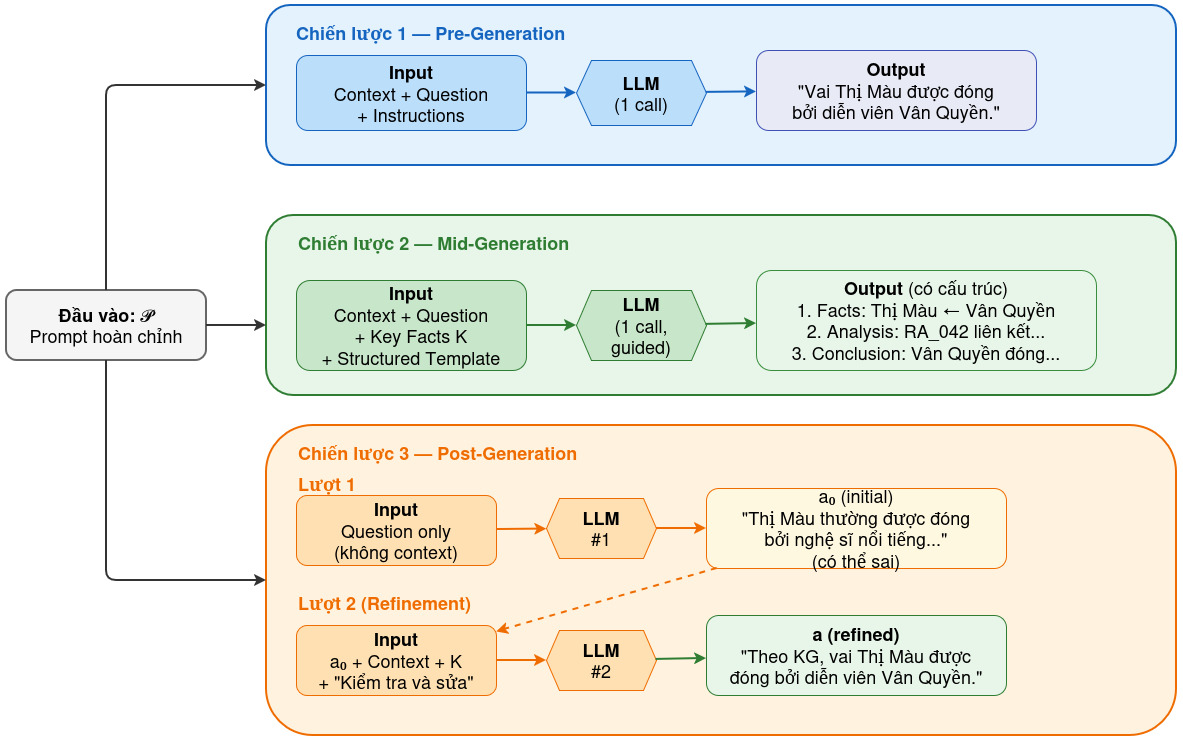
\includegraphics[width=\textwidth]{figures/c3/generation_strategies.jpg}
  \caption{Ba chiến lược tạo sinh.}
  \label{fig:generation_strategies}
\end{figure}


\subsubsection{Kiểm soát ảo giác}

Hiện tượng ảo giác (\textit{hallucination}) --- việc LLMs sinh thông tin không có căn cứ trong ngữ cảnh được cung cấp --- là rủi ro thường thấy khi tích hợp mô hình ngôn ngữ vào hệ thống truy vấn tri thức có tính ràng buộc cao. Phân hệ G-Generation triển khai cơ chế kiểm soát hai lớp để giảm thiểu rủi ro này (\textbf{Hình \ref{fig:hallucination_control}}).

\textbf{Lớp 1 --- Phòng ngừa trước tạo sinh (pre-generation).} Các biện pháp phòng ngừa được tích hợp trực tiếp vào cấu trúc prompt trước khi gọi LLMs:
\begin{itemize}
  \item \textit{Entity Catalog Grounding}: Tại giai đoạn tiền xử lý truy vấn (Query Processing), prompt \texttt{QUERY\_EXPAND\_AND\_EXTRACT} chứa sẵn danh mục thực thể hợp lệ từ Knowledge Graph. LLMs chỉ được phép trích xuất các thực thể thuộc danh mục này, ràng buộc hệ thống ngay từ bước đầu tiên chỉ tham chiếu các đối tượng có thực trong đồ thị tri thức.
  \item \textit{Key Facts Injection}: Dữ kiện chính $K$ được đặt ở vị trí ưu tiên cao trong prompt (ngay sau Context Header), định hướng quá trình suy luận theo các sự kiện đã được xác minh từ đồ thị tri thức trước khi mô hình trả lời câu hỏi.
  \item \textit{Chỉ dẫn ràng buộc}: Mỗi template tạo sinh (\texttt{PRE\_GENERATION}, \texttt{POST\_REFINE}) đều chứa chỉ dẫn tường minh yêu cầu LLMs trích dẫn ``tên riêng chính xác từ dữ liệu graph'', thu hẹp không gian sinh của mô hình về phạm vi ngữ cảnh được cung cấp.
\end{itemize}

\textbf{Lớp 2 --- Phát hiện và sửa trong quá trình tạo sinh (in-generation).} Các cơ chế can thiệp được nhúng vào chính quy trình tạo sinh:
\begin{itemize}
  \item Với chiến lược Mid, template cấu trúc ba phần buộc mô hình trích xuất dữ kiện cụ thể trước khi đưa ra kết luận (\textit{facts} $\rightarrow$ \textit{analysis} $\rightarrow$ \textit{conclusion}). Chuỗi suy luận tường minh này tạo điều kiện cho việc kiểm tra tính nhất quán giữa bằng chứng và kết luận.
  \item Với chiến lược Post, lượt gọi thứ hai đối chiếu tường minh câu trả lời sơ bộ $a_0$ với dữ liệu thực tế từ Knowledge Graph. Template \texttt{POST\_REFINE} yêu cầu mô hình thực hiện ba bước rõ ràng: kiểm tra $a_0$ với dữ liệu, sửa lỗi nếu có, và bổ sung chi tiết cụ thể --- bao gồm cả ví dụ minh họa cách cải thiện để mô hình nắm rõ kỳ vọng.
\end{itemize}

Lớp phòng ngừa hạn chế xác suất sinh thông tin sai ngay từ đầu; lớp phát hiện can thiệp trong quá trình tạo sinh, đặc biệt hiệu quả với chiến lược Post khi có cơ chế đối chiếu hai lượt tường minh.

\begin{figure}[ht]
  \centering
  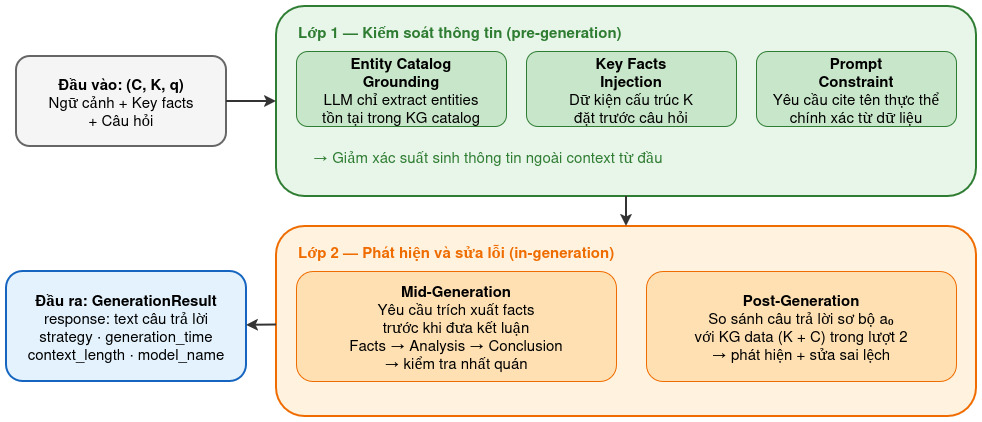
\includegraphics[width=\textwidth]{figures/c3/hallucination_control.jpg}
  \caption{Cơ chế hai lớp kiểm soát chất lượng.}
  \label{fig:hallucination_control}
\end{figure}


\section{Thiết kế bộ dữ liệu đánh giá (Benchmark)}

\subsection{Nguyên tắc xây dựng bộ dữ liệu đánh giá}

Để đánh giá hiệu quả của hệ thống một cách khách quan và có kiểm soát, một bộ dữ liệu đánh giá chuyên biệt được xây dựng dựa trên đóng góp của các chuyên gia trong lĩnh vực Chèo cùng tri thức có trong Knowledge Graph. Bộ dữ liệu được xây dựng ưu tiên (i) \textit{tính chính xác}, (ii)\textit{tính đại diện} và (iii)\textit{khả năng đo lường rõ ràng}, tương tự các nghiên cứu về benchmark cho hệ thống hỏi đáp dựa trên tri thức có cấu trúc \cite{peng2025m3gqa}.

Bộ dữ liệu đánh giá được xây dựng theo 4 nguyên tắc chính. Thứ nhất là \textit{tính hiện thực} (realism), trong đó mọi thực thể và quan hệ xuất hiện trong câu hỏi đều tồn tại trong Knowledge Graph, đảm bảo rằng hệ thống có đủ tri thức để trả lời. Thứ hai là \textit{tính toàn diện} (coverage), các câu hỏi được thiết kế để bao phủ nhiều loại truy vấn khác nhau, đặc biệt bao gồm các truy vấn yêu cầu suy luận đa bước, vốn được xem là thách thức cốt lõi trong các hệ thống KGQA hiện đại \cite{wang2023multihop}. Thứ ba là \textit{tính đo lường được} (measurability), mỗi câu hỏi đều có ground truth rõ ràng nhằm hỗ trợ đánh giá định lượng. Cuối cùng là \textit{tính cân bằng} (balance), đảm bảo phân bố hợp lý giữa các mức độ phức tạp của truy vấn.

Bộ kiểm thử gồm 100 câu hỏi được xây dựng thủ công và nhận cố vấn từ các chuyên gia về nghệ thuật Chèo nhằm đảm bảo tính chính xác. Mặc dù số lượng không lớn, thiết kế tập trung vào độ phức tạp quan hệ và khả năng suy luận, phù hợp với xu hướng benchmark hiện đại nhấn mạnh reasoning thay vì chỉ retrieval \cite{peng2025m3gqa}.

\subsection{Phân loại truy vấn}

Các câu hỏi trong bộ câu hỏi đánh giá được phân loại thành ba nhóm: Local, Community và Global. Việc phân loại này được xây dựng dựa trên ba tiêu chí chính: (i) \textit{phạm vi truy xuất trong đồ thị}, (ii) \textit{độ phức tạp suy luận đa bước} và (iii) \textit{đặc trưng của kiến trúc GraphRAG}.

Xét theo phạm vi truy xuất, các nghiên cứu về GraphRAG cho thấy sự khác biệt rõ rệt giữa truy vấn cục bộ và truy vấn toàn cục. Edge et al. \cite{edge2024graphrag} chỉ ra rằng các hệ thống Retrieval-Augmented Generation truyền thống chủ yếu phù hợp với các truy vấn cục bộ, trong đó thông tin cần thiết có thể được truy xuất từ một số lượng nhỏ các đoạn văn bản hoặc thực thể liên quan. Ngược lại, các truy vấn toàn cục yêu cầu tổng hợp thông tin từ toàn bộ tập dữ liệu, tương ứng với bài toán tóm tắt theo truy vấn (query-focused summarization), vượt ra ngoài khả năng của các phương pháp truy xuất cục bộ. Trên cơ sở đó, GraphRAG đề xuất các cơ chế truy xuất ở nhiều mức độ, bao gồm local search và global search. Từ góc nhìn này, có thể xác định thêm một mức trung gian là community-level, trong đó truy vấn yêu cầu khai thác thông tin trong một cụm thực thể có liên kết chặt chẽ trong đồ thị. Mức này phản ánh cấu trúc tự nhiên của Knowledge Graph, nơi các thực thể thường được tổ chức thành các cộng đồng (communities) thông qua các quan hệ ngữ nghĩa.

Xét theo độ phức tạp suy luận, các truy vấn trong hệ thống hỏi đáp tri thức thường yêu cầu suy luận qua nhiều bước (multi-hop reasoning), trong đó câu trả lời được suy ra thông qua chuỗi các quan hệ trong đồ thị \cite{wang2023multihop}. Các nghiên cứu gần đây cho thấy hiệu năng của hệ thống phụ thuộc đáng kể vào khả năng xử lý các truy vấn multi-hop, đặc biệt khi số lượng bước suy luận tăng lên \cite{shah2024multihop}. Do đó, việc phân loại truy vấn theo số bước suy luận là cần thiết để đánh giá hệ thống một cách toàn diện.

Hiện nay, các benchmark hiện đại cho hệ thống GraphRAG nhấn mạnh rằng việc đánh giá cần bao phủ nhiều mức độ truy vấn khác nhau, từ truy vấn đơn giản đến truy vấn yêu cầu tổng hợp tri thức phức tạp \cite{peng2025m3gqa}. Điều này nhằm đảm bảo rằng hệ thống không chỉ hoạt động tốt ở các trường hợp đơn giản mà còn có khả năng xử lý các truy vấn có cấu trúc quan hệ phức tạp.

Trên cơ sở các tiêu chí trên, các truy vấn trong bộ kiểm thử được phân loại như sau:

\textbf{Local queries} (35\%) là các truy vấn yêu cầu truy xuất thông tin trực tiếp từ một hoặc một số ít thực thể trung tâm, với số bước suy luận nhỏ (thường từ một đến hai bước).

\begin{tcolorbox}[colback=gray!5, colframe=black!50, arc=4pt, boxrule=0.5pt]
{\small
\begin{verbatim}
{
  "id": "CASE_014",
  "category": "local_queries",
  "subcategory": "direct_relation",
  "question": "Ai đóng vai Nô trong vở Quan Âm Thị Kính?",
  "ground_truth": {
    "answer": "Văn Quân và Mạnh Phóng đóng vai Nô.",
    "related_entities": ["Văn Quân", "Mạnh Phóng", "Nô", 
                        "Quan Âm Thị Kính"]
  }
}
\end{verbatim}
}
\end{tcolorbox}
Truy vấn trên có thể được biểu diễn dưới dạng một chuỗi quan hệ ngắn trong đồ thị tri thức, bắt đầu từ thực thể vở diễn, liên kết đến nhân vật, sau đó tới vai diễn và cuối cùng là nghệ sĩ biểu diễn. Toàn bộ quá trình truy xuất được giới hạn trong một vùng lân cận nhỏ của đồ thị và không yêu cầu tổng hợp thông tin từ nhiều nguồn khác nhau. Do đó, truy vấn này đại diện cho lớp bài toán truy xuất cục bộ, trong đó câu trả lời có thể được xác định thông qua một truy vấn đồ thị đơn với số bước duyệt hữu hạn.

\textbf{Community queries} (32\%) là các truy vấn yêu cầu kết nối nhiều thực thể trong cùng một cụm quan hệ và tổng hợp thông tin từ nhiều đường dẫn trong đồ thị.

\begin{tcolorbox}[colback=gray!5, colframe=black!50, arc=4pt, boxrule=0.5pt]
{\small
\begin{verbatim}
{
  "id": "CASE_051",
  "category": "community_queries",
  "subcategory": "play_cast",
  "question": "Những diễn viên nào đã tham gia đồng thời 
               cả vở Quan Âm Thị Kính và Kim Nham?",
  "ground_truth": {
    "answer": "An Chinh, Tuấn Kha, Bá Dũng, Huy Toàn, Ngọc Minh",
    "related_entities": ["Quan Âm Thị Kính", "Kim Nham"]
  }
}
\end{verbatim}
}
\end{tcolorbox}
Trong truy vấn này, hệ thống cần thực hiện hai quá trình truy xuất độc lập để xác định tập các nghệ sĩ tham gia từng vở diễn, sau đó kết hợp các kết quả thông qua phép giao tập hợp. Về mặt cấu trúc, truy vấn bao gồm nhiều đường dẫn trong đồ thị xuất phát từ các thực thể khác nhau, và không thể được giải quyết bằng một truy vấn cục bộ đơn lẻ. Điều này cho thấy truy vấn yêu cầu khai thác một cụm thực thể có liên kết chặt chẽ, đồng thời thực hiện tổng hợp thông tin ở mức trung gian.

\textbf{Global queries} (33\%) là các truy vấn yêu cầu tổng hợp thông tin từ nhiều phần khác nhau của Knowledge Graph và đòi hỏi suy luận đa bước trên phạm vi rộng.

\begin{tcolorbox}[colback=gray!5, colframe=black!50, arc=4pt, boxrule=0.5pt]
{\small
\begin{verbatim}
{
  "id": "CASE_083",
  "category": "global_queries",
  "subcategory": "thematic_synthesis",
  "question": "So sánh số phận bi kịch của Súy Vân và Thị Kính?",
  "ground_truth": {
    "answer": "...",
    "related_entities": ["Súy Vân", "Thị Kính"]
  }
}
\end{verbatim}
}
\end{tcolorbox}

Khác với hai nhóm trước, truy vấn này không chỉ yêu cầu truy xuất thực thể và quan hệ, mà còn đòi hỏi tổng hợp và diễn giải thông tin từ nhiều phần khác nhau của đồ thị tri thức. Hệ thống cần khai thác các tiểu đồ thị liên quan đến từng nhân vật, bao gồm các mối quan hệ, sự kiện và bối cảnh, sau đó kết hợp các thông tin này để đưa ra một nhận định mang tính khái quát. Do đó, truy vấn thuộc loại toàn cục, trong đó truy xuất tri thức và tạo sinh ngôn ngữ đóng vai trò bổ trợ lẫn nhau, phù hợp với mô hình query-focused summarization trong GraphRAG \cite{edge2024graphrag}.

Việc phân loại truy vấn theo ba mức Local, Community và Global cho phép đánh giá hệ thống một cách có cấu trúc theo từng cấp độ truy xuất và suy luận, đồng thời phản ánh đúng đặc trưng của các hệ thống GraphRAG hiện đại.

\subsection{Mức độ bao phủ của bộ dữ liệu}

Bộ dữ liệu đánh giá được thiết kế để khai thác tri thức trong Knowledge Graph Chèo một cách toàn diện, trải dài từ tầng thực thể cụ thể đến tầng suy luận trừu tượng về chủ đề nghệ thuật.

Ở \textit{tầng thực thể}, bộ câu hỏi chạm tới đủ cả năm loại thực thể chính của ontology --- vở chèo, nhân vật, diễn viên, trích đoạn và phiên bản biểu diễn. Mỗi loại đều xuất hiện vừa ở vai trò chủ thể truy vấn (``Ai đóng vai X?'', ``Vở Y có những trích đoạn nào?'') vừa ở vai trò ngữ cảnh trả lời, qua đó đảm bảo hệ thống phải thực sự duyệt qua toàn bộ cấu trúc node-type của đồ thị thay vì chỉ tập trung vào một vài kiểu thường gặp. 

Ở \textit{tầng quan hệ}, các câu hỏi buộc hệ thống phải đi qua hầu hết các object property của ontology, từ \texttt{performedBy}, \texttt{forCharacter} cho quan hệ diễn viên--vai diễn, cho đến \texttt{hasCharacter}, \texttt{hasScene}, \texttt{hasVersion} và \texttt{inVersion} cho cấu trúc vở--trích đoạn--phiên bản. Nhiều câu hỏi cần phối hợp nhiều property liên tiếp, chẳng hạn truy vấn ``diễn viên nào đóng vai Tuần Ty trong trích đoạn Tuần Ty--Đào Huế của vở Chu Mãi Thần'' đòi hỏi chuỗi bốn bước truy cập đồ thị để trả về đúng cá thể.

Ở \textit{tầng nội dung}, bộ câu hỏi bao phủ nhiều lớp thông tin đặc thù của nghệ thuật Chèo: thông tin tiểu sử và tính cách nhân vật; các mối quan hệ xã hội (vợ--chồng, mẹ--con, bạn hữu, và các xung đột đạo đức); cấu trúc nghệ thuật của vở diễn cùng dàn diễn viên qua từng phiên bản; sự nghiệp diễn xuất của nghệ sĩ trải dài trên nhiều vở; các chủ đề và biểu tượng nghệ thuật (oan khuất, hy sinh, triết lý Phật giáo, hình tượng người phụ nữ trong xã hội phong kiến); cũng như hệ phân loại nhân vật truyền thống của chèo (Đào, Kép, Hề, Lão). Đặc biệt, các câu hỏi không bị bó hẹp trong phạm vi một vở --- nhiều câu hỏi yêu cầu so sánh và tổng hợp liên vở (như đối chiếu số phận bi kịch giữa các nhân vật nữ chính, hay truy vết sự nghiệp của những diễn viên tham gia đồng thời nhiều vở). Dạng truy vấn này buộc hệ thống xây dựng ngữ cảnh toàn cục thay vì chỉ dựa vào một vùng lân cận nhỏ của đồ thị, qua đó phơi bày điểm yếu cốt lõi của các kiến trúc RAG truyền thống vốn chỉ tối ưu cho truy vấn cục bộ~\cite{edge2024graphrag}.

Bên cạnh các lớp tri thức phổ biến, bộ câu hỏi còn bao phủ một số tình huống đặc thù của miền nghệ thuật biểu diễn sống: cùng một vai diễn có thể được nhiều diễn viên thể hiện trong các phiên bản khác nhau, trong khi cùng một kiểu nhân vật (như Hề) có thể xuất hiện trong nhiều trích đoạn thuộc các vở khác nhau nhưng được mô hình hóa như những cá thể độc lập trong đồ thị. Việc hệ thống phải nhận diện và phân biệt chính xác các trường hợp này chính là bài kiểm tra trực tiếp dành cho khả năng xử lý mẫu reification --- một thiết kế then chốt của ontology Chèo được kế thừa.

\section*{Tiểu kết}
\addcontentsline{toc}{section}{Tiểu kết}
Chương này đã trình bày quá trình phân tích và thiết kế kiến trúc GraphRAG cho miền nghệ thuật Chèo, tổ chức theo hai tầng tách biệt là tầng tri thức và tầng xử lý logic. Cách phân tầng này đảm bảo khả năng kiểm soát tri thức thông qua Knowledge Graph và duy trì tính minh bạch của quá trình suy luận.

Ở tầng tri thức, ontology Chèo được kế thừa và chuẩn hóa thành Knowledge Graph trên Neo4j, kèm các cơ chế suy luận quan hệ gián tiếp ở mức ứng dụng và chiến lược lập chỉ mục chuyên biệt nhằm khắc phục hạn chế của OWL reasoner thuần túy, đáp ứng yêu cầu truy vấn thời gian thực. Ở tầng xử lý logic, phân hệ G-Retrieval được xây dựng theo hướng đa độ hạt để xử lý linh hoạt nhiều dạng truy vấn, còn phân hệ G-Generation tích hợp tri thức có kiểm soát với prompt đóng vai trò trung tâm điều hướng quá trình sinh và hạn chế hiện tượng ảo giác.

Bên cạnh phần thiết kế kiến trúc, chương cũng xây dựng bộ dữ liệu đánh giá CheoBench v2 với cách phân tầng truy vấn Local, Community, Global tương ứng với đặc trưng của GraphRAG --- làm công cụ đi kèm phục vụ cho việc triển khai và đánh giá thực nghiệm ở chương tiếp theo.